% !TEX root = thesis-ex.tex

\section{The Large Hadron Collider}

The Large Hadron Collider (LHC) is part of the European Organization for Nuclear Research. It has a circumference of 27 kilometers, making it the world's largest particle accelerator, and is housed in a tunnel that is up to 175 meters below the surface of the earth. The LHC has eight arcs and eight straight sections, with each straight section being approximately 528 m long. The arc sections are built using 1232 dipole superconducting magnets, providing a magnetic field of up to 8.33 T. Another 392 quadrupole magnets are used for focussing the beam. The magnets are cooled down to 1.9 K via liquid Helium. The LHC beam pipe has two rings with counter-rotating beams and uses a uses a twin-bore magnet design that optimizes for both cost, as well as space. The counterrotating beams require opposite magnetic dipole fields in both rings, with separate magnetic and vacuum chambers, with the common sections only at the insertion regions, where the major experimental detectors are located. These detectors are: A Toroidal LHC Apparatus (ATLAS), Compact Muon Solenoid (CMS), A Large Ion Collider Experiment (ALICE), and Large Hadron Collider - Beauty (LHCb) \cite{Evans:2008zzb}.

Capable of reaching up to center of mass energies, \sqrts\ = 14 TeV for protons and \sqrtsnn\ = 5.5 TeV for lead ions, the LHC delivers up to $10^{34} \mathrm{cm}^2\mathrm{s}^1$ of luminosity to the ATLAS and CMS detectors when colliding protons. The LHCb detector is a lower luminosity experiment, that receives up to $10^{32} \mathrm{cm}^2\mathrm{s}^1$, and ALICE, a dedicated ion experiment aims at a peak luminosity of $10^{27} \mathrm{cm}^2\mathrm{s}^1$ for nominal lead-lead operation. The beams in the LHC are accelerated by 16 radio frequency (RF) cavities that provide a voltage of 2 MV and operate at 400 MHz. They consist of bunches of protons or ions that are kept in their circular path by the dipole magnets, and focussed via the quadrupole magnets, 

%It has two transfer tunnels, approximately 2.5 km in length, that connect it to the accelerator complex shown in Fig.~\ref{fig:cern}. Built in the tunnel originally used for the Large Electron-Positron Collider, the LHC was designed to collide protons at center of mass energies of up to 14 TeV. It 

A schematic of the entire accelerator complex and the path followed by protons and heavy ions is show in Fig.~\ref{fig:cern}.  Protons are obtained by stripping the hydrogen atom of its electrons via an electric field. The complete ionization of lead is done in multiple stages, with the first stage providing for $\mathrm{Pb}^{+29}$ via an ion source. Both the protons and heavy ions are then are accelerated by increasingly powerful accelerators, until they reach the main LHC beam pipes. Protons start at LINAC 2 (LINear ACcelerator), whereas the lead ions start at LINAC 3. The $\mathrm{Pb}^{+29}$ lead ions are further stripped of electrons by passing them through a 0.3 $\mu$m foil after the LINAC 3. The $\mathrm{Pb}^{+54}$ ions are selected via mass spectrometer and sent to the Low Energy Ion Ring (LEIR), whereas the protons are sent to the Booster. They are then sent to the Proton Synchrotron (PS), followed by the Super Proton Synchrotron (SPS), and then finally the LHC. The final stripping of lead ions takes place after the PS, on a 0.8 mm thin aluminum foil.

%The LHC beams consist of 
%The LHC delivered an integrated luminosity of 0.49 \pb\ of \pbpb\ and 25 \pb\ of \pp\ data in 2015.

\begin{figure}[ht]
	\centering
	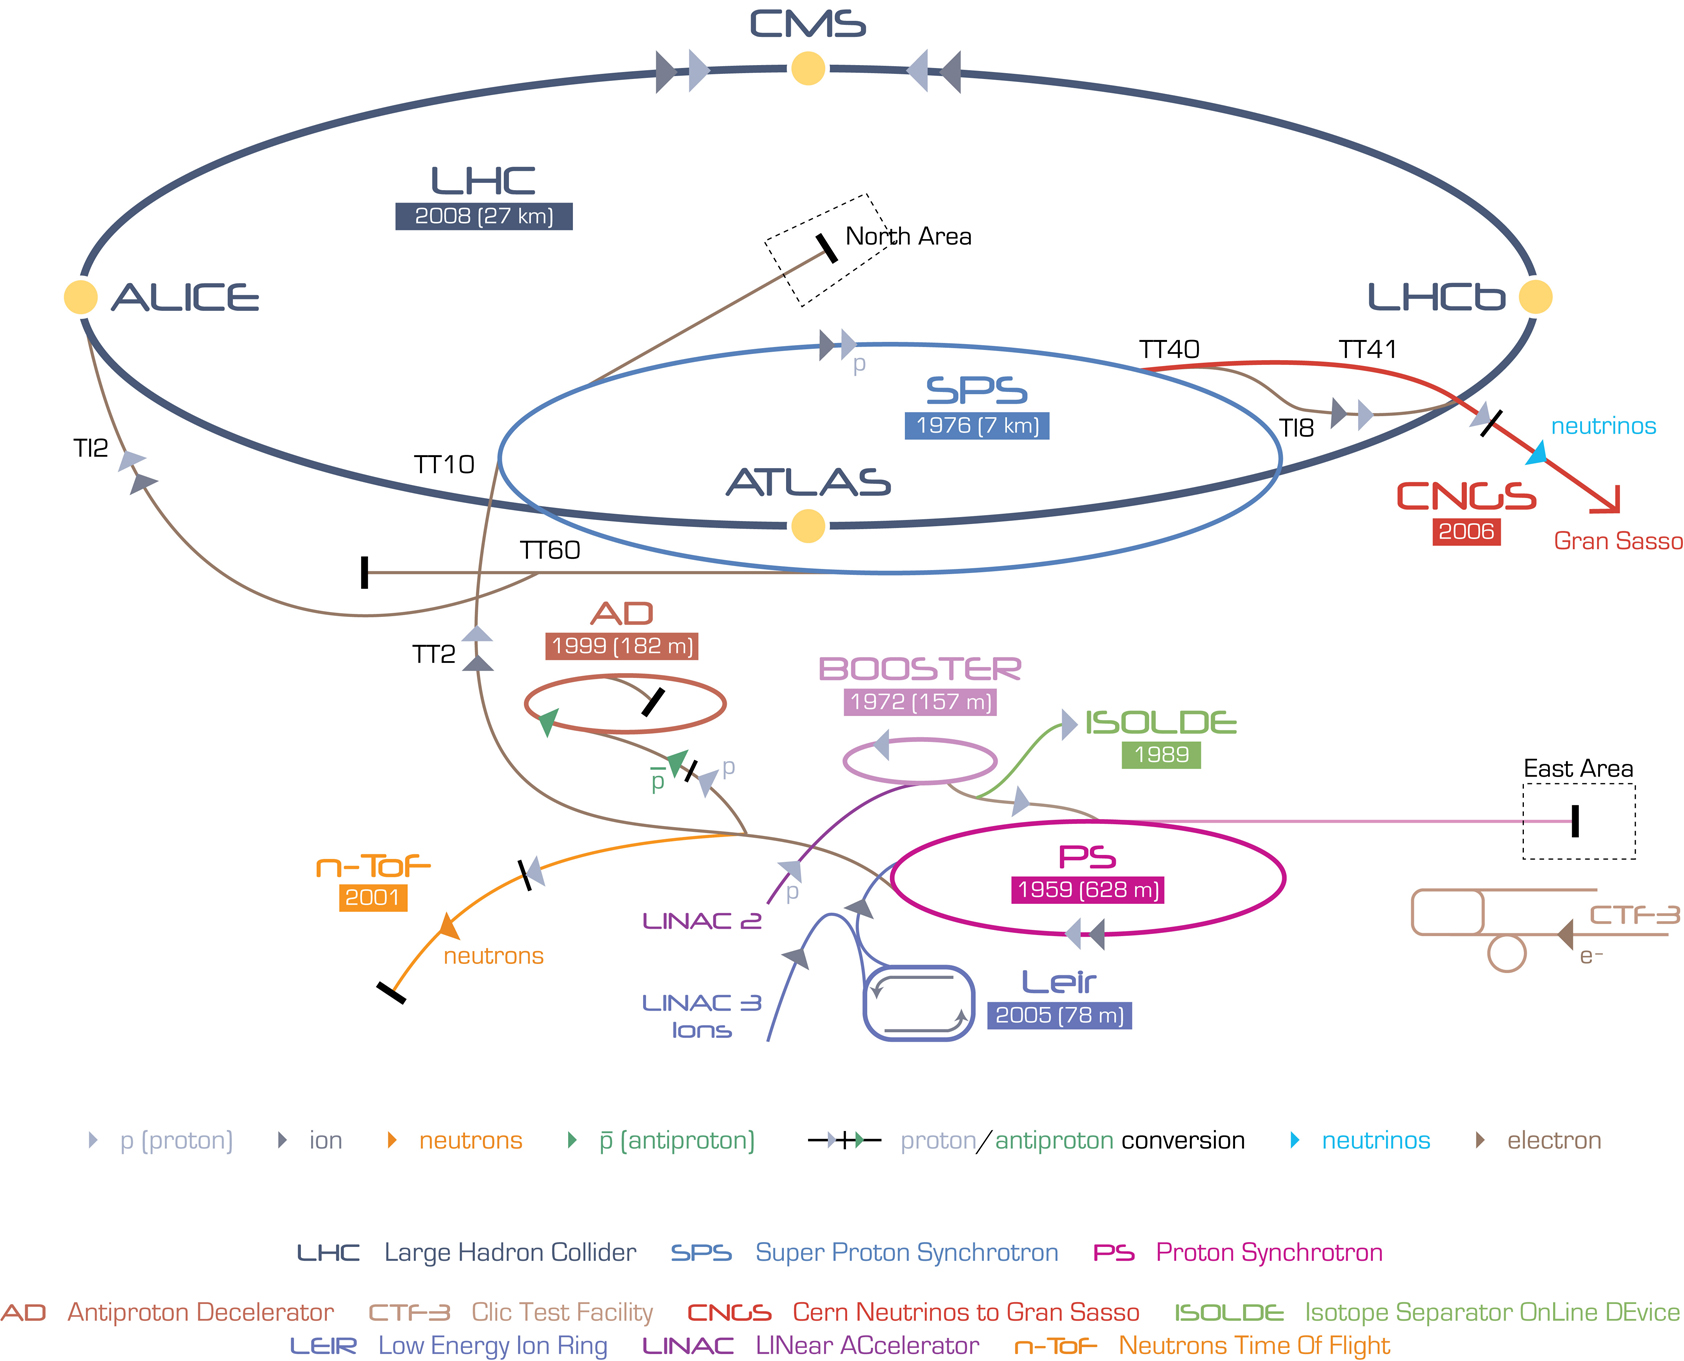
\includegraphics[width=1.\textwidth]{figures/cern.jpg} %
	\caption{The accelerator complex at CERN. ATLAS can be seen inside the SPS on the LHC ring. Figure taken from Ref.~\cite{TEEPCLPC}}
	\label{fig:cern}%
\end{figure}


%%%%%%%%%%YK%%%%%%%%

%During the LHC's first operational data taking run, referred to as Run 1 (2009-2013), the first collisions with stable beams were observed between protons and protons (\pp), as well as protons with lead ions (\pPb) at center of mass energies of \sqrts=8 TeV and \sqrtsnn=2.76 TeV, respectively. Center of mass energies for \pPb\ collisions were subsequently increased to \sqrtsnn=5.02 TeV in 2013. After an extended technical shutdown for upgrades following Run 1, the LHC was restarted for run Run 2, during which \pp\ and \pPb\ collisions with stable beams were observed at center-of-mass energies of \sqrts=13 TeV and \sqrtsnn=8.16 TeV, respectively. 
%
%The LHC is located in a tunnel at depths of 50 to 175 m underground. Originally, this tunnel was built for the Large Electron-Proton Collider (LEP), an electron-proton collider that was operation from 1989-2000. In the LHC, particle packets in high vacuum beam pipes going in opposite directions are accelerated by 8 radio frequency cavities (RF) which deliver voltages up to 2 MV at an oscillator frequency of 400 MHz. Each 26.7 km ring consists of eight arched sections with 616 dipole super-conducting magnets per beam, which supply fields of up to 8.33 Tesla. An additional 196 beam focusing quadropole magnets per beam serve to narrow the beam and increase luminosity. To supply such high magnetic fields, LHC magnets use super-fluid helium and operate at temperatures down to 1.9 K while the RF cavities operate at temperatures down to 4.5 K.
%
%Any proton or lead ion entering the LHC must go through the complex chain of accelerators shown in  Fig.~\ref{fig:cern}. In order to be accelerated and focused in the beams, the proton and lead ions are required to have a net positive charge. Thus, the hydrogen and lead atoms must be first stripped of the electrons in their atomic shells. Positively charged protons are obtained by stripping atoms of hydrogen gas from their electrons using an electric field. Positively charged lead ions are initially extracted from a source which provides partially stripped lead ions with an average around $\mathrm{Pb^{29+}}$. These ions then go through a series of pre-accelerators, seen at the bottom of Fig.~\ref{fig:cern}, starting with the Linear Accelerator 3 (LINAC3) where they are further stripped of electrons by passing through $3.0\ \mu$m  of carbon foil. Next, a mass spectrometer selects lead ions with an average $\mathrm{Pb^{29+}}$ to be fed into the Low Energy Ion Ring (LEIR). The protons, meanwhile, begin their journey at the Linear Accelerator 2 (LINAC2). Both protons and lead ions then enter the next phase of pre-accelerators which consist of the Proton Synchrotron (PS) and the Super Proton Synchrotron (SPS), where they continue to be  accelerated. The lead ions are completely stripped away of remaining electrons at the exit of the PS, where they pass through 0.8 mm aluminum foil. The final stage is at the exit of the SPS where the protons and lead ions enter the LHC for the final phase of acceleration before they are collided.
% 
%Beams in the LHC consist of 2808 bunches of protons or lead ions with bunch spacing down to 25 ns (7.5 m). A proton bunch contains approximately 1.15x$10^{11}$ protons while an ion bunch contains approximately 2.2x$10^{8}$ ions. These beams are brought to collide at four interaction points which can be seen along the circumference of the LHC in Fig.~\ref{fig:cern}. At these interaction points there are detectors present to analyze the collisions: A Large Ion Collider Experiment (ALICE), A Toroidal LHC Apparatus (ATLAS), Compact Muon Solenoid (CMS), and the Large Hadron Collider Beauty (LHCb).
%%%%%%%%%%YKend%%%%%%%%


\section{The ATLAS Detector}

The ATLAS detector (Fig.~\ref{fig:atlas}) is a general purpose detector at the LHC. It is symmetric in the forward-backward direction, and has a full $2\pi$ coverage in azimuth. It uses a right-handed coordinate system with its origin at the nominal interaction point (IP) in the centre of the detector and the $z$-axis along the beam pipe. The $x$-axis points from the IP to the centre of the LHC ring, and the $y$ axis points upward. Cylindrical coordinates $(r,\phi)$ are used in the transverse plane, $\phi$ being the azimuthal angle around the beam pipe. The pseudorapidity is defined in terms of the polar angle $\theta$ as $\eta=-\ln\tan(\theta/2)$.}

The A side of the detector is defined as having positive $z$, withe C side being defined as having negative $z$. 

It has three main subsystems: the inner detector, the calorimeter, and the muon spectrometer. This paper will only discuss the inner detector and the calorimeter, since those are the systems that will be used in the analysis.

\footnote{
ATLAS uses a 

\begin{figure}[ht]
	\centering
	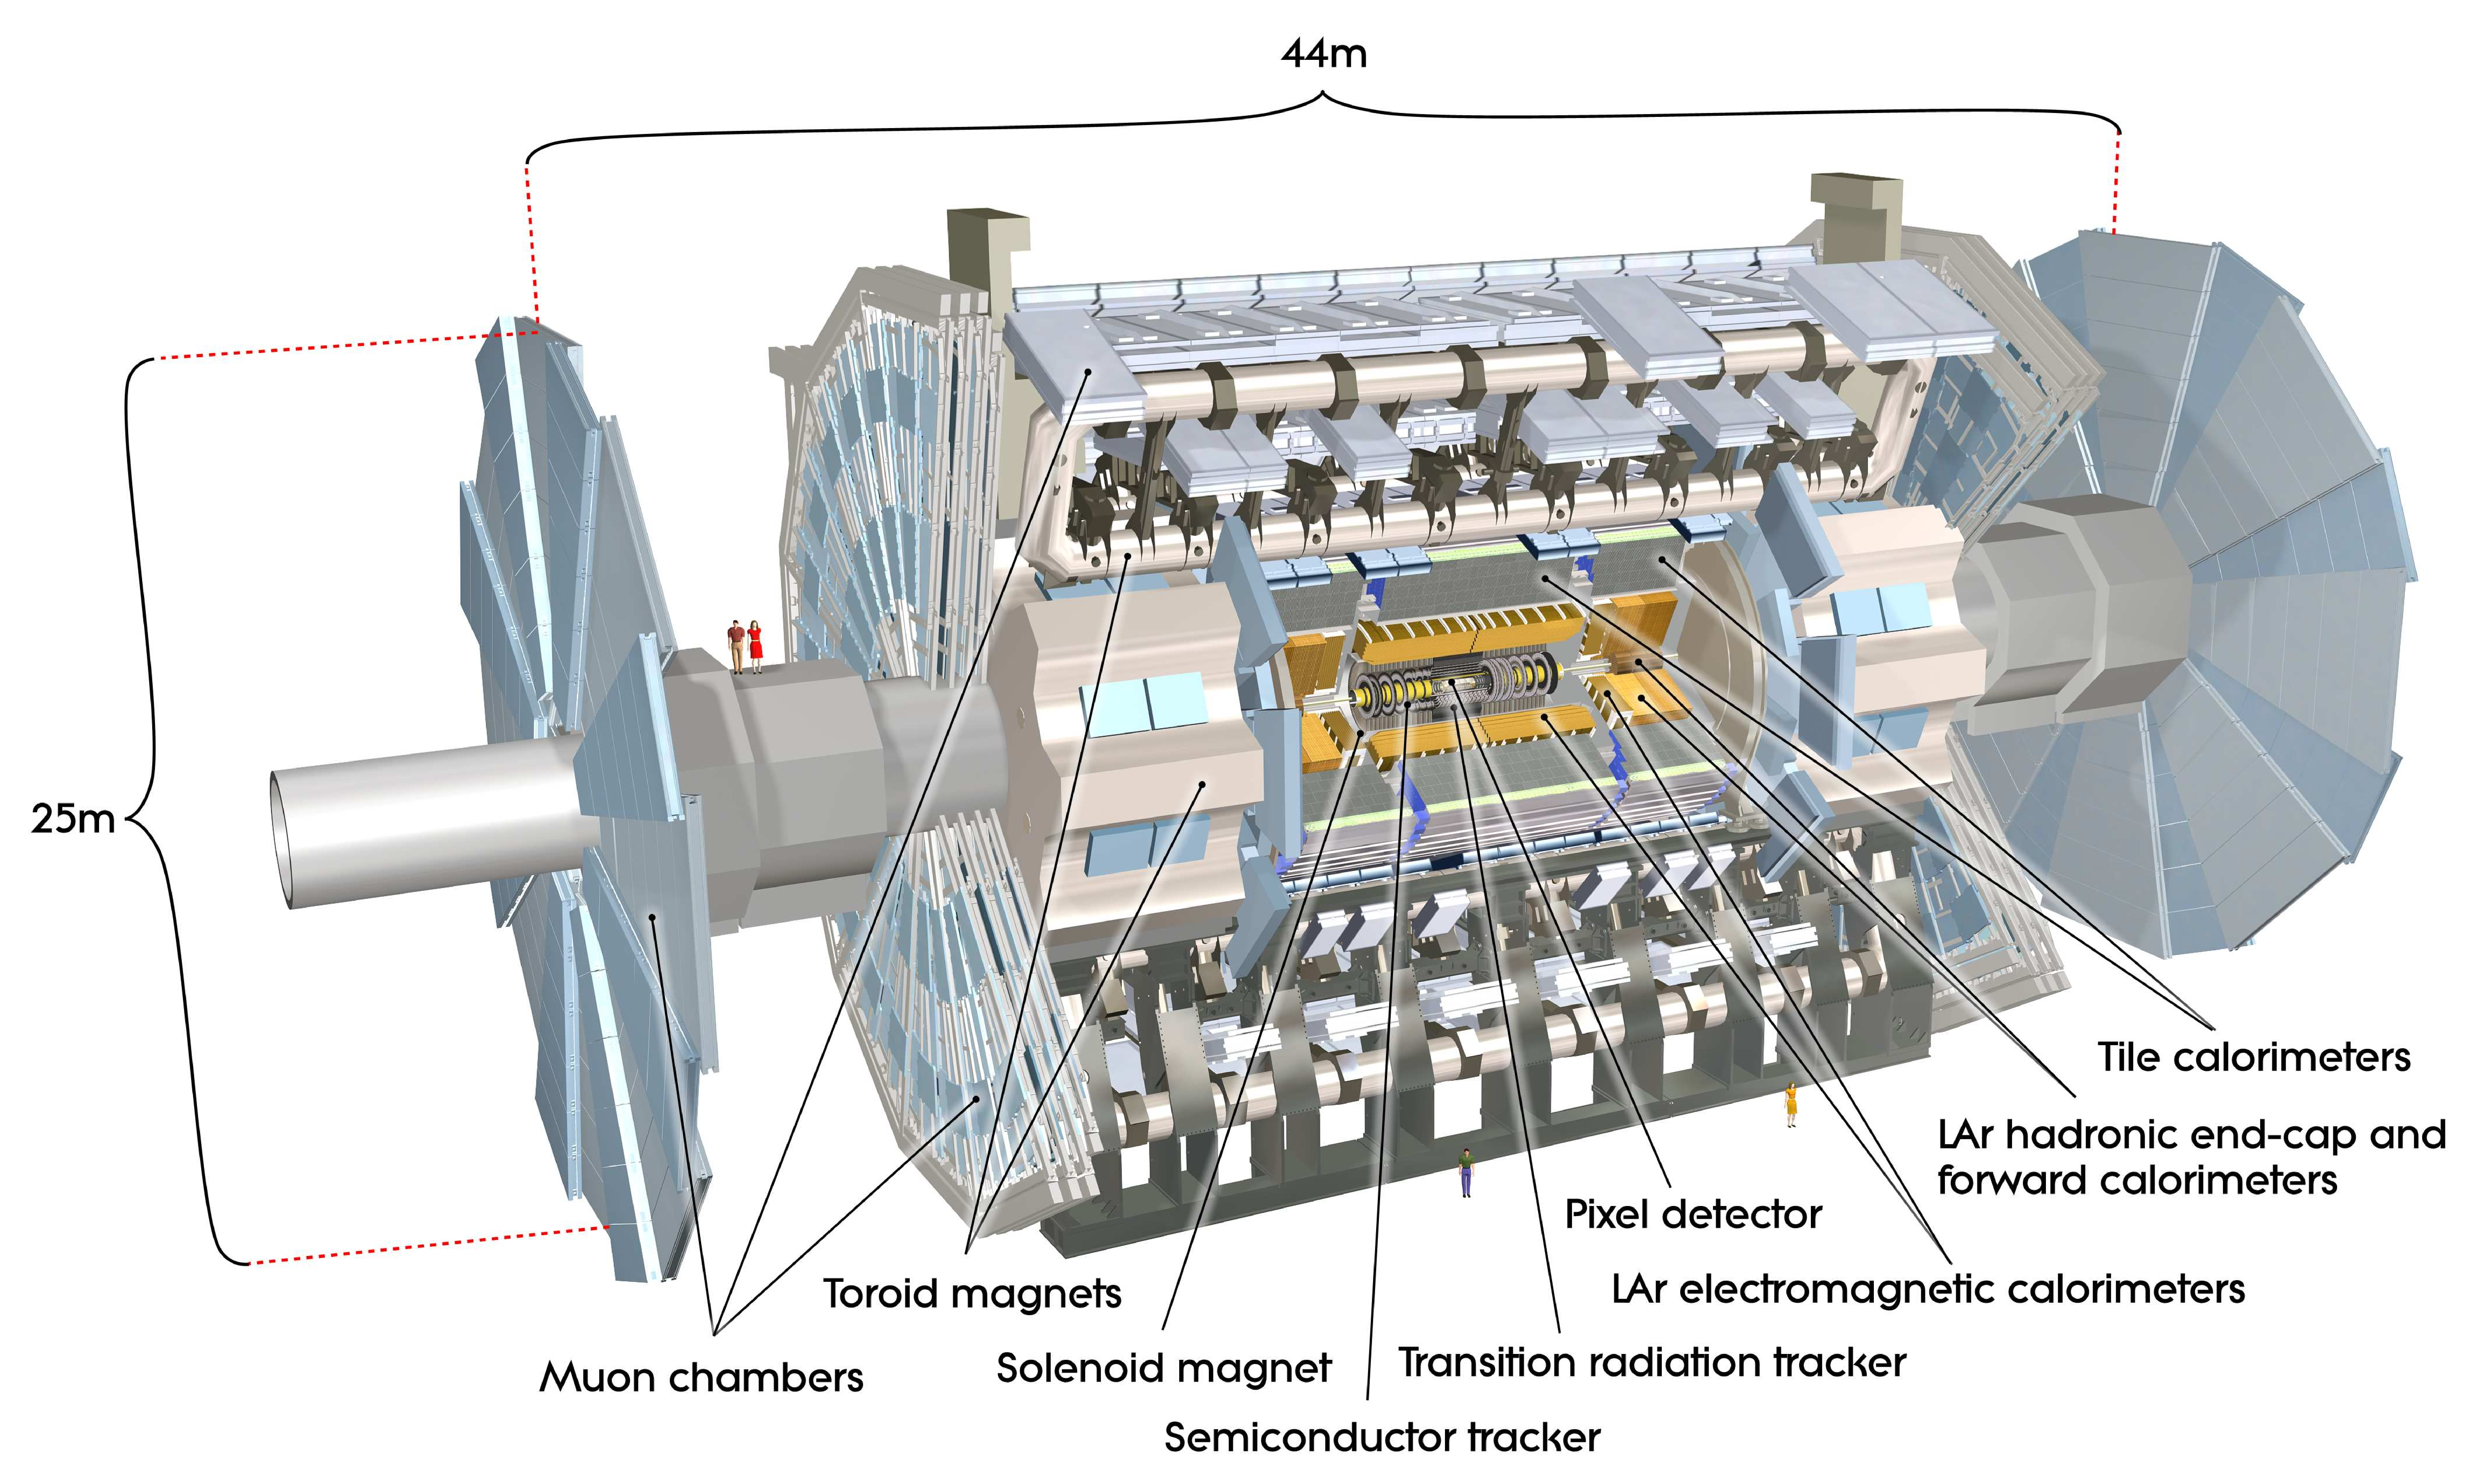
\includegraphics[width=0.7\textwidth]{figures/atlas.pdf} %
	\caption{The ATLAS detector. Figure taken from Ref.~\cite{Aad:2008zzm}.}	
	\label{fig:atlas}%
\end{figure}


\subsubsection{Inner Detector}
The inner detector (Fig.~\ref{fig:inner_det}) is designed to reconstruct the charged particle trajectories in the interval $|\eta| < 2.5$ . This is achieved by a combination of three subsystems: the Pixel detector, the Semiconductor Tracker (SCT), and the straw-tube Transition Radiation Tracker (TRT), all immersed in a 2T magnetic field \cite{Aad:2008zzm}.

The pixel detector consists of four layers of pixels, with the innermost layer at a distance of 33.25 mm from the interaction point. The expected hit resolution of the pixel detector ranges from of $\sim$ 8$\mu$m ($\sim$ 40$\mu$m) in $r-\phi$ ($z$) \cite{ibl_design} for the innermost layer, to $\sim$ 10$\mu$m ($\sim$ 115$\mu$m) in $r-\phi$ ($z$) for the next three layers \cite{Aad:2008zzm}.

The SCT has eight strip (80 $\mu$m pitch) layers that are crossed by each track. Small angle stereo strips are used to measure both coordinates, with one set of strips in each layer, parallel to the beam direction. The end cap region has nine layers of double sided modules with strips in the radial direction, with each also having a mean pitch of 80 $\mu$m. The intrinsic resolution is $\sim$ 17$\mu$m ($\sim$ 580$\mu$m) in $r-\phi$ ($z$)  \cite{Aad:2008zzm}.

The TRT contains 73 (160) layers of straws and fibers in the barrel (end-cap), and provides a large number of hits per track, allowing track-following for $|\eta| <  2.0$. T. It has a resolution of $\sim$ 130$\mu$m in $r-\phi$, with no information in the $z$ direction \cite{Aad:2008zzm}.

 \begin{figure}[htbp!]
    \centering
      \begin{subfigure}{0.44\textwidth}
        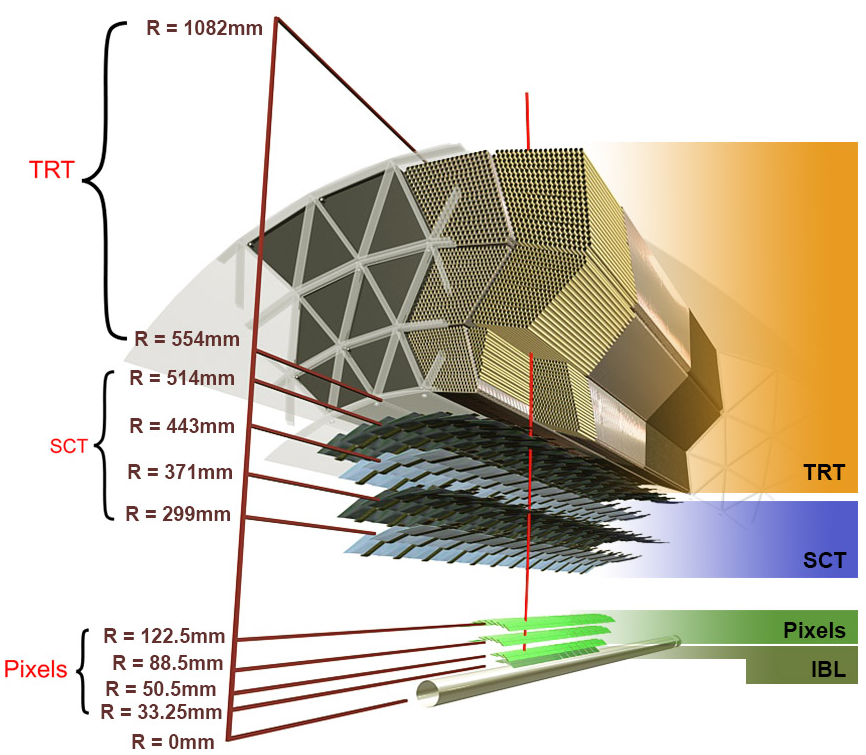
\includegraphics[width=\textwidth]{inner_det.png}
          \caption{ATLAS Inner Detector System}
          \label{fig:inner_det}
      \end{subfigure}
      \hfill
      \begin{subfigure}{0.49\textwidth}
        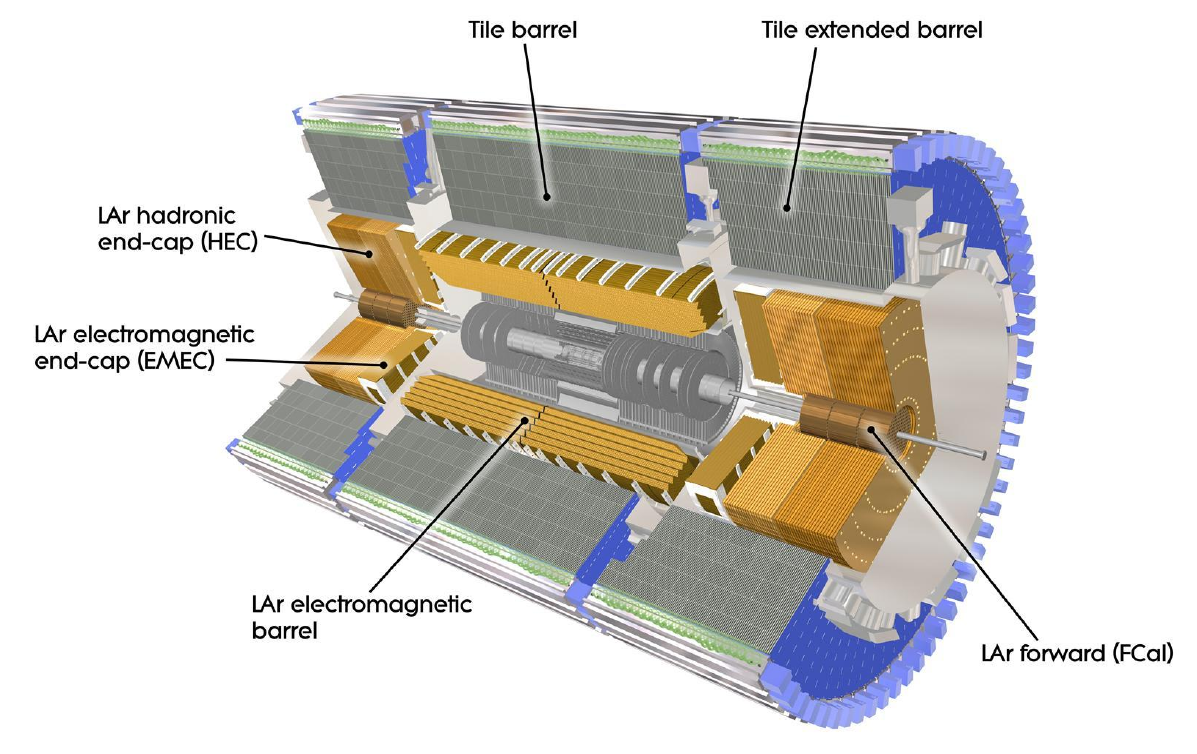
\includegraphics[width=\textwidth]{calorimeters.png}
          \caption{A cut-away view of the ATLAS calorimeter system. Taken from \cite{Aad:2008zzm}}
          \label{fig:cal}
      \end{subfigure}
\caption{
\label{fig:atlas_systems}%
ATLAS Inner detector and calorimeter systems}
\end{figure}


\subsubsection{Calorimeter}
The calorimeter system (Fig.~\ref{fig:cal}) covers the region $|\eta| < 4.9$, using different techniques over different ranges.

The sampling liquid argon (LAr) electromagnetic calorimeter (EMCal) covers $|\eta| < 3.2$ (the barrel region for $|\eta| < 1.475$ and two end caps for $1.375 < |\eta| < 3.2$) . Its accordion-like geometry provides full $\phi$ symmetry without azimuthal cracks. The EMCal is segmented longitudinally into three layers, plus a pre-sampler, with the granularity varying as a function of layer depth and pseudorapidity. The presampler ($|\eta| <1.8$) compensates for the energy lost by photons and electrons upstream of the calorimeter \cite{Aad:2008zzm}.  

The hadronic calorimeters (HCal) consist of the Tile, Hadronic End Cap (HEC), and the Forward Calorimeters (FCal). The Tile is placed directly outside the EMCal, covering $|\eta| < 1.0$, with the extended barrels covering the range $0.8 <|\eta|< 1.7$. It uses steel as the absorber and scintillating tiles as the active material. It has three layers, with the two sides of the tiles being read out by wavelength shifting fibers into separate photomultiplier tubes. The HEC consists of two wheels per cap, and is directly behind the EMCal end cap. It covers $1.5< |\eta| < 3.2$, overlapping both the tile and the FCal (at $|\eta| =  3.1$). The active material in the HEC is LAr (with copper plates acting as the absorber). The FCal, ranging from $3.1 < |\eta| < 4.9$, consists of three modules in each end cap; the first, made of copper, is optimized for electromagnetic interactions, while the other two, made of tungsten, are optimized for hadronic measurements \cite{Aad:2008zzm}.


\iffalse
The $\eta$ coverage of the different detector systems can be seen in Fig.~\ref{fig:atlaspseudorap}.
\begin{figure}[htbp!]
	\centering
	\includegraphics[width=0.7\textwidth]{atlaspseudorap.png} %
	\caption{$\eta$ acceptance of the ATLAS detector.}	
	\label{fig:atlaspseudorap}%
\end{figure}
\fi











\begin{figure}[ht]
	\centering
	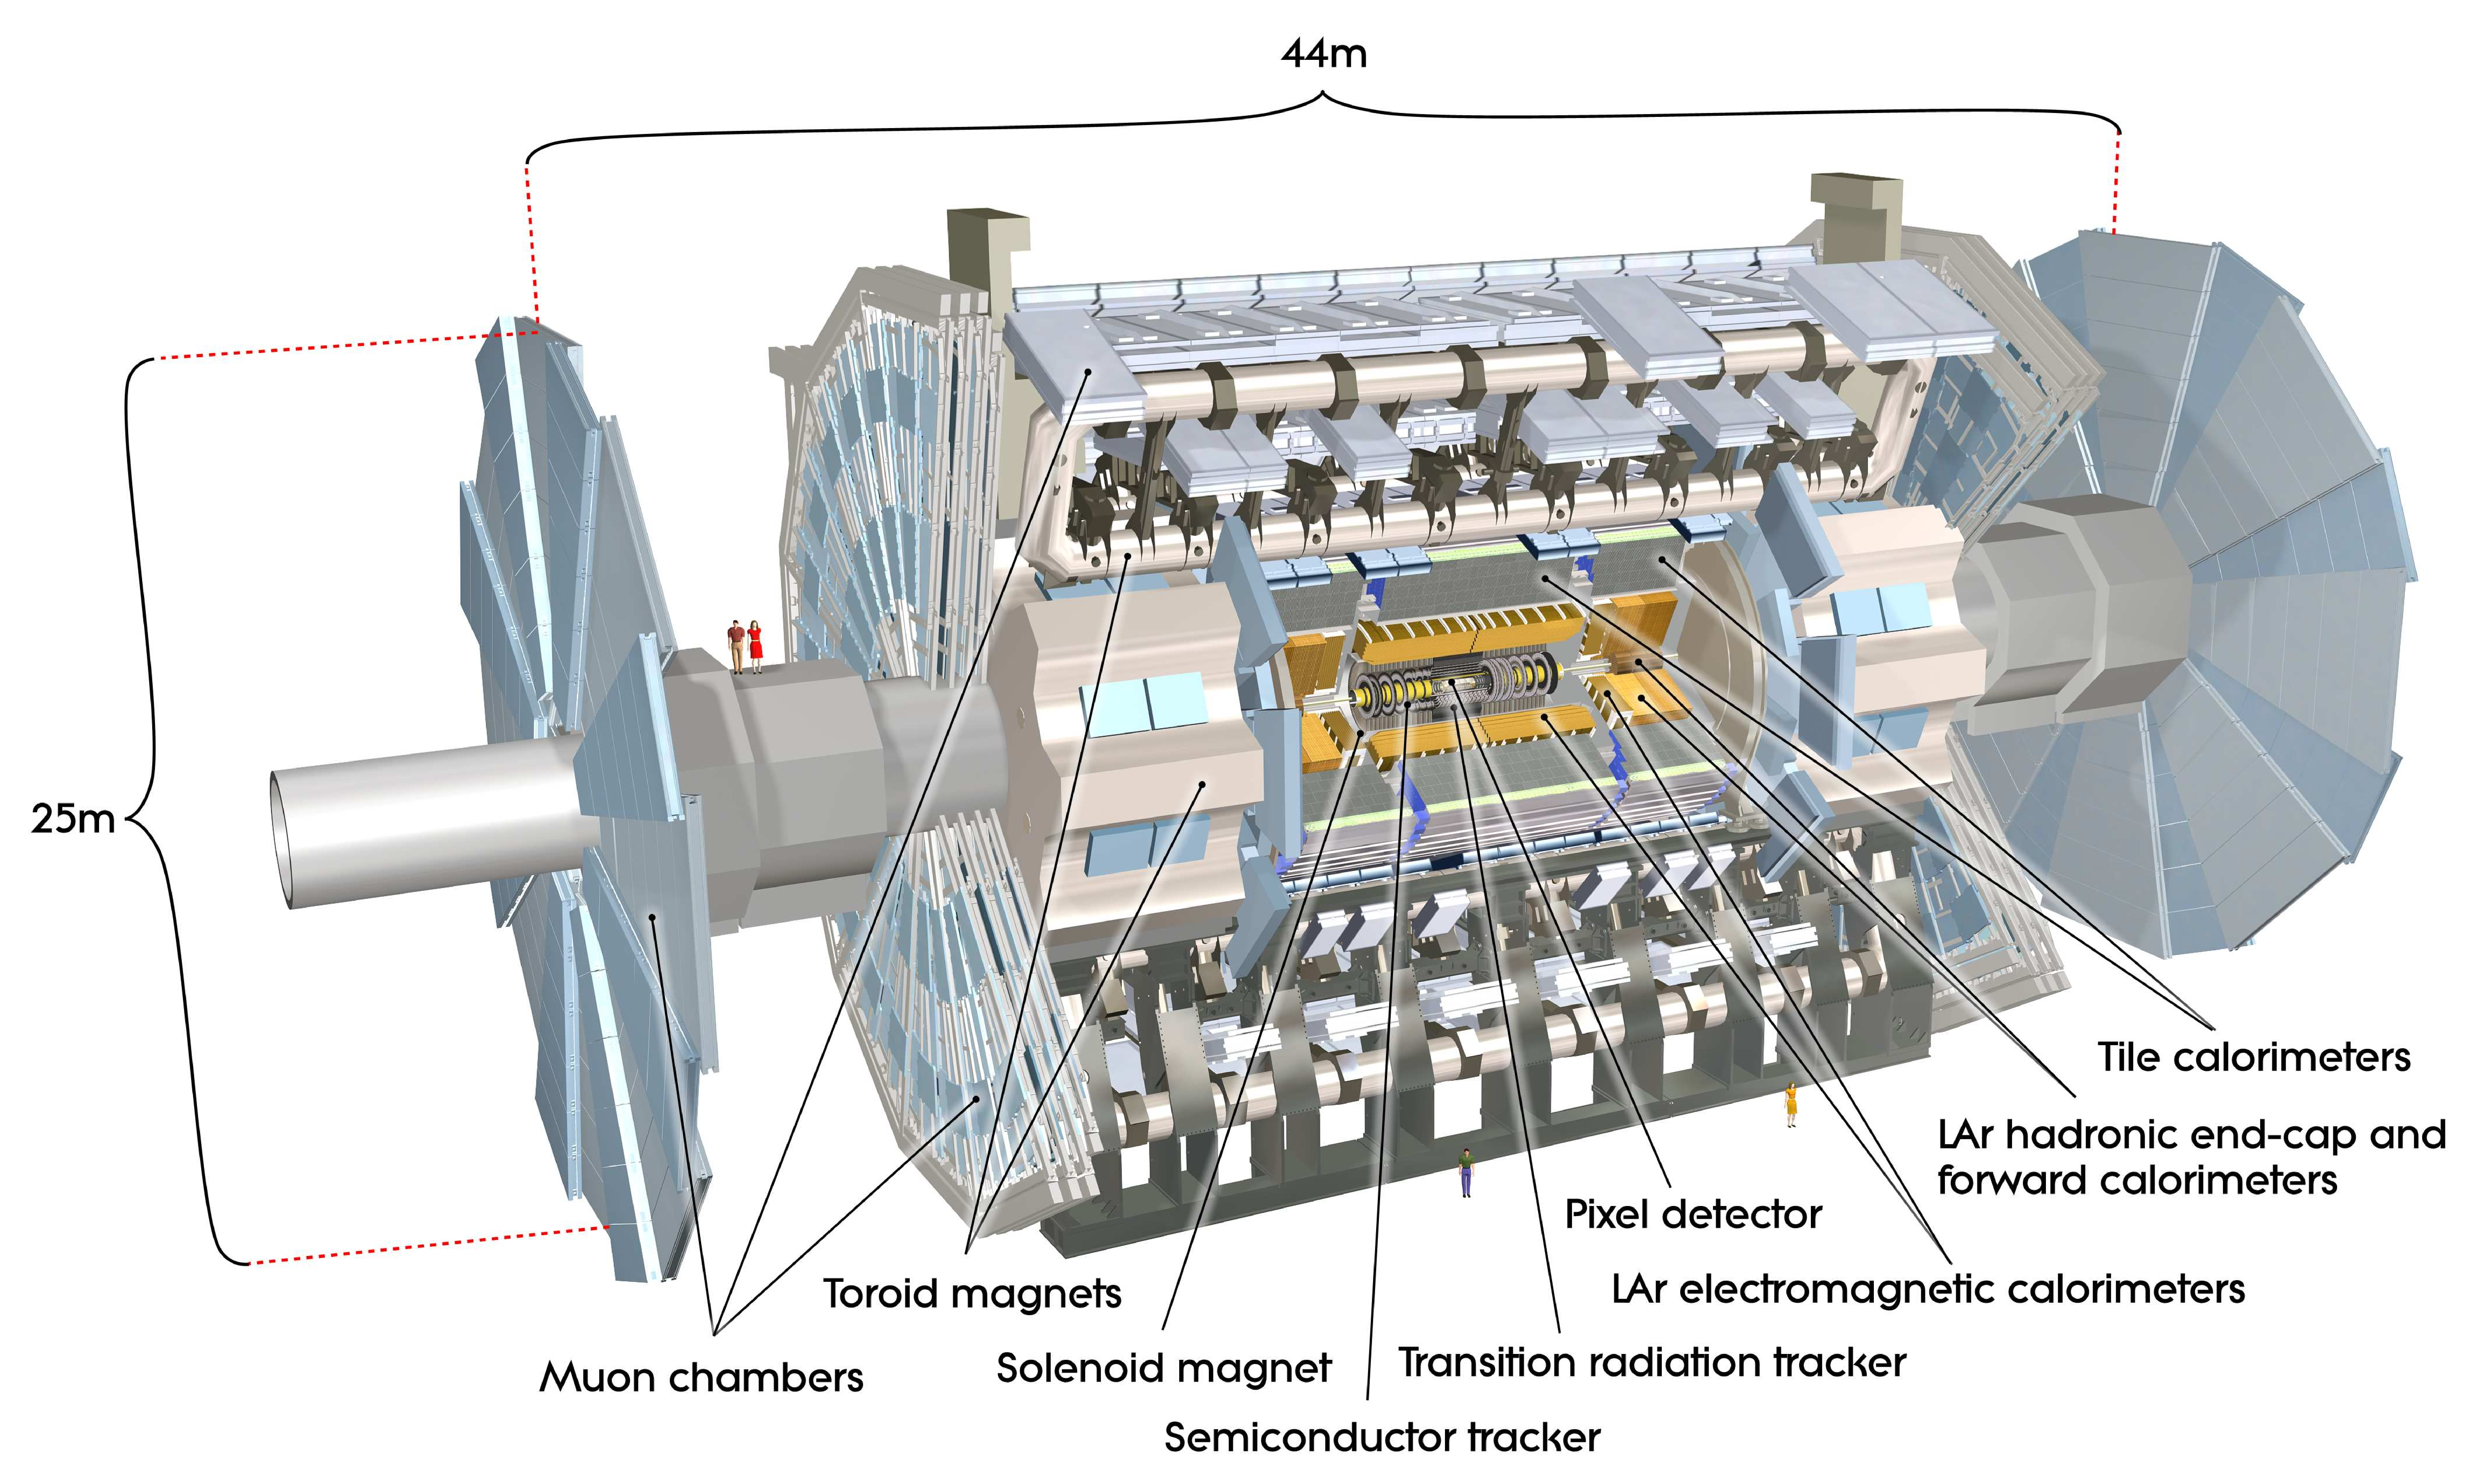
\includegraphics[width=0.7\textwidth]{figures/atlas.pdf} %
	\caption{The ATLAS detector. Figure taken from Ref.~\cite{Aad:2008zzm}.}	
	\label{fig:atlas}%
\end{figure}

The ATLAS detector~\cite{Aad:2008zzm}, shown in Fig.~\ref{fig:atlas} is one of the two larger detectors on the LHC and is located at interaction point 1 (IP1) on the LHC ring\footnote{
	ATLAS uses a right-handed coordinate system with its origin at the nominal interaction point (IP) in the centre of the detector and the $z$-axis along the beam pipe. The $x$-axis points from the IP to the centre of the LHC ring, and the $y$ axis points upward. Cylindrical coordinates $(r,\phi)$ are used in the transverse plane, $\phi$ being the azimuthal angle around the beam pipe. The pseudorapidity is defined in terms of the polar angle $\theta$ as $\eta=-\ln\tan(\theta/2)$. Angular distance is measured in units of $\Delta R \equiv \sqrt{(\Delta\eta)^{2} + (\Delta\phi)^{2}}$. Rapidity is defined in terms of energy and momentum of a particle or jet as $y=\frac{1}{2}ln(\frac{E+p_{z}}{E-p_{z}})$. The rapidity with center-of-mass frame boost accounted for is denoted \ystar.} 
It is designed to perform measurements of Standard Model physics, including the search for the Higgs boson, and search for physics beyond the Standard Model. Although ATLAS is primarily a detector used to measure $pp$ collisions, it has also been used to study Heavy Ion physics with much higher nuclear collision energies and much larger particle multiplicities compared to \pp\ collision.

\begin{figure}
	\centering
	\includegraphics[width=0.7\textwidth]{figures/atlaspseudorap.png} %
	\caption{ ATLAS detector pseudorapidity coverage. All components cover $2\pi$ in azimuth. }	
	\label{fig:atlasrap}%
\end{figure}

The ATLAS detector consists of four main parts, or sub-detectors. The closest part to the interaction point is the Inner Detector (ID), which is placed close to the IP and is used to measure charged particle tracks. The ID is inside a 2 Tesla solenoidal magnetic field, which causes charged particles to curve, allowing their momentum to be measured. Outside of the ID are the electromagnetic (EM) and hadronic calorimeters. These give energy measurements and are the primary detectors for the analysis presented in this thesis. The fourth and outermost part is the muon spectrometer which is placed inside a toroidal field provided by eight toroid magnets. The muon system is the outermost part of the detector because due to their weakly interacting nature, muons are one of the only particles which pass through the calorimeters. All of the ATLAS sub-detectors have full $2\pi$ azimuthal coverage and different pseudorapidity coverages shown in  Fig.~\ref{fig:atlasrap}. A detailed description of the ATLAS detector and it's subsystems can be found in~\cite{Aad:2008zzm}. 

\subsection{ATLAS Trigger System}
\label{sec:trigger}

In order to select events during data-taking, a complex hardware and software system called the $trigger$ is required. It relies on many detector subsystems to flag events based on a set of rules that are defined prior to each run. A two-level trigger system was used to select the \pp\ and \pPb\ collisions analyzed for the measurement presented in this thesis. The first, the hardware-based trigger stage Level-1 (L1), is implemented with custom electronics. The second level is the software-based High Level Trigger (HLT). The HLT consists of the Level-2 (L2) trigger, followed by the event filter (EF). The ATLAS trigger was designed for a collision rate of 40 MHz, with the L1 trigger designed to reduce the rate to 75 kHz, and the HLT to perform a final reduction to about 200 Hz, which is the final even rate written to disk. A schematic of the ATLAS trigger and data acquisition systems can be seen in Fig.~\ref{fig:trigdaq}. Some triggers selecting minimum-bias (MB) events used the minimum-bias trigger scintillator detectors (MBTS). The MBTS detect charged particles over $2.1 < |\eta| < 3.9$ using two segmented counters placed at $z = \pm 3.6$~m. Each counter provides measurements of both the pulse heights and the arrival times of ionization energy deposits~\cite{Aad:2008zzm}.

\begin{figure}[t]
	\centerline{
		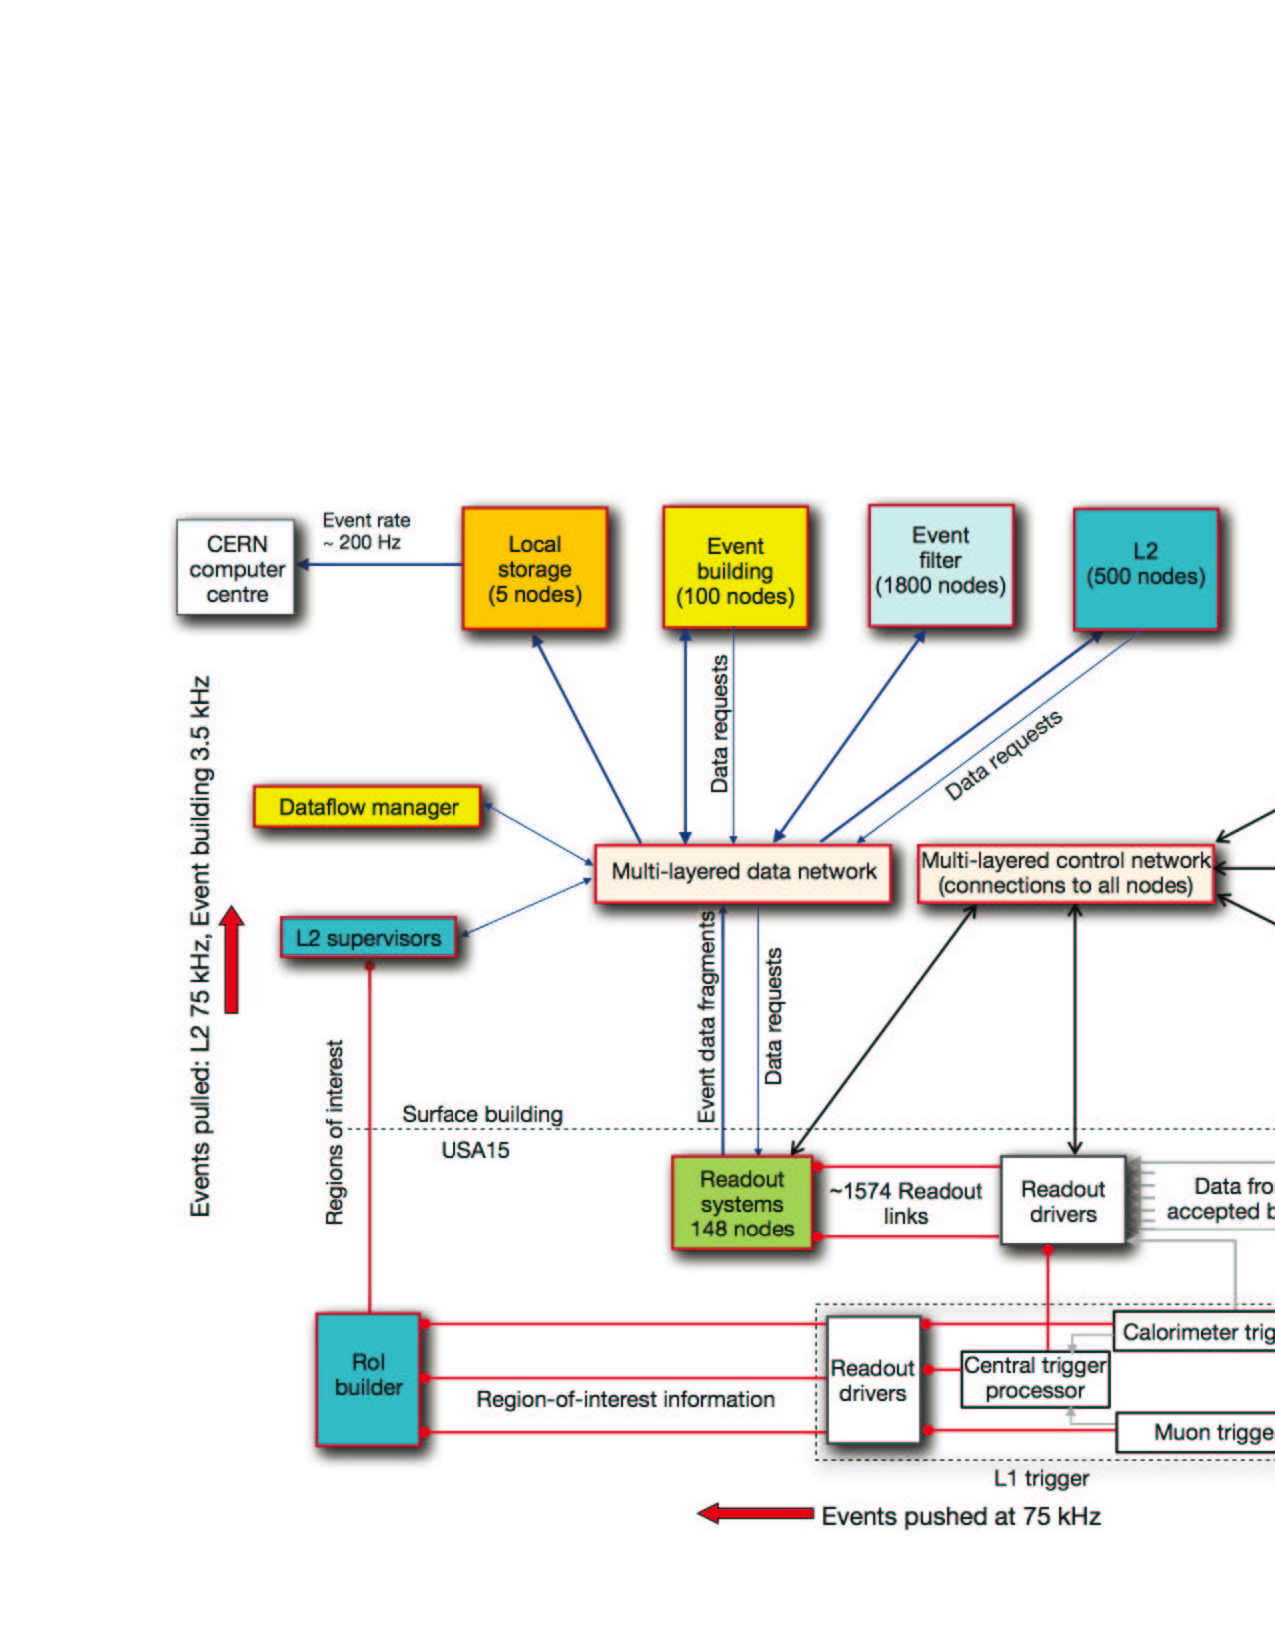
\includegraphics[width=0.52\textwidth]{figures/trig_daq.pdf} %
		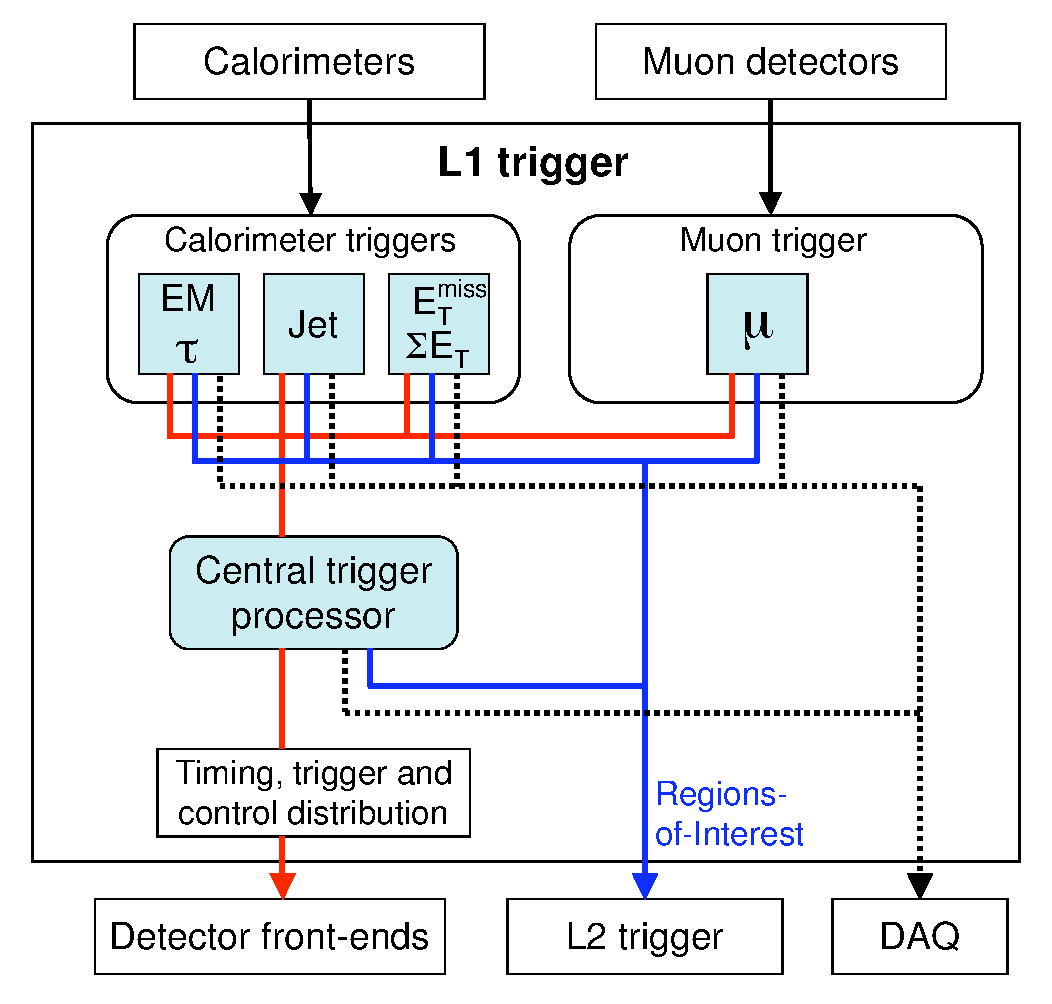
\includegraphics[width=0.48\textwidth]{figures/trig_l1.pdf} %
	}
	\caption{ A schematic (left) of the ATLAS trigger and data acquisition systems, and the L1 hardware trigger (right). The total event rate of about 40 MHz is reduced by the L1 trigger to about 75 kHz, and further reduced to 200 Hz by the HLT (L2 + EF) trigger.Figure taken from Ref.~\cite{Aad:2008zzm}.}	
	\label{fig:trigdaq}
\end{figure}

Some triggers can be prescaled, meaning that not every event meeting the requirements of a particular trigger is saved to disk. If a trigger with prescale $c_{p}$ is saved $n$ times, this corresponds to $c_{p}n$ events passing through the HLT. The decision of what prescale to assign to a trigger is very complicated. Various physics analysis groups have different requirements, but unfortunately not all data from a run can be saved due to technical limitations. Depending on the physics goals of a particular run, the trigger menu, which assigns the triggers and their respective prescales, will change. The UIUC ATLAS group has been responsible for the trigger system operation in all of the heavy ion runs since 2015.


\subsection{Calorimetery}

\begin{figure}
	\centering
	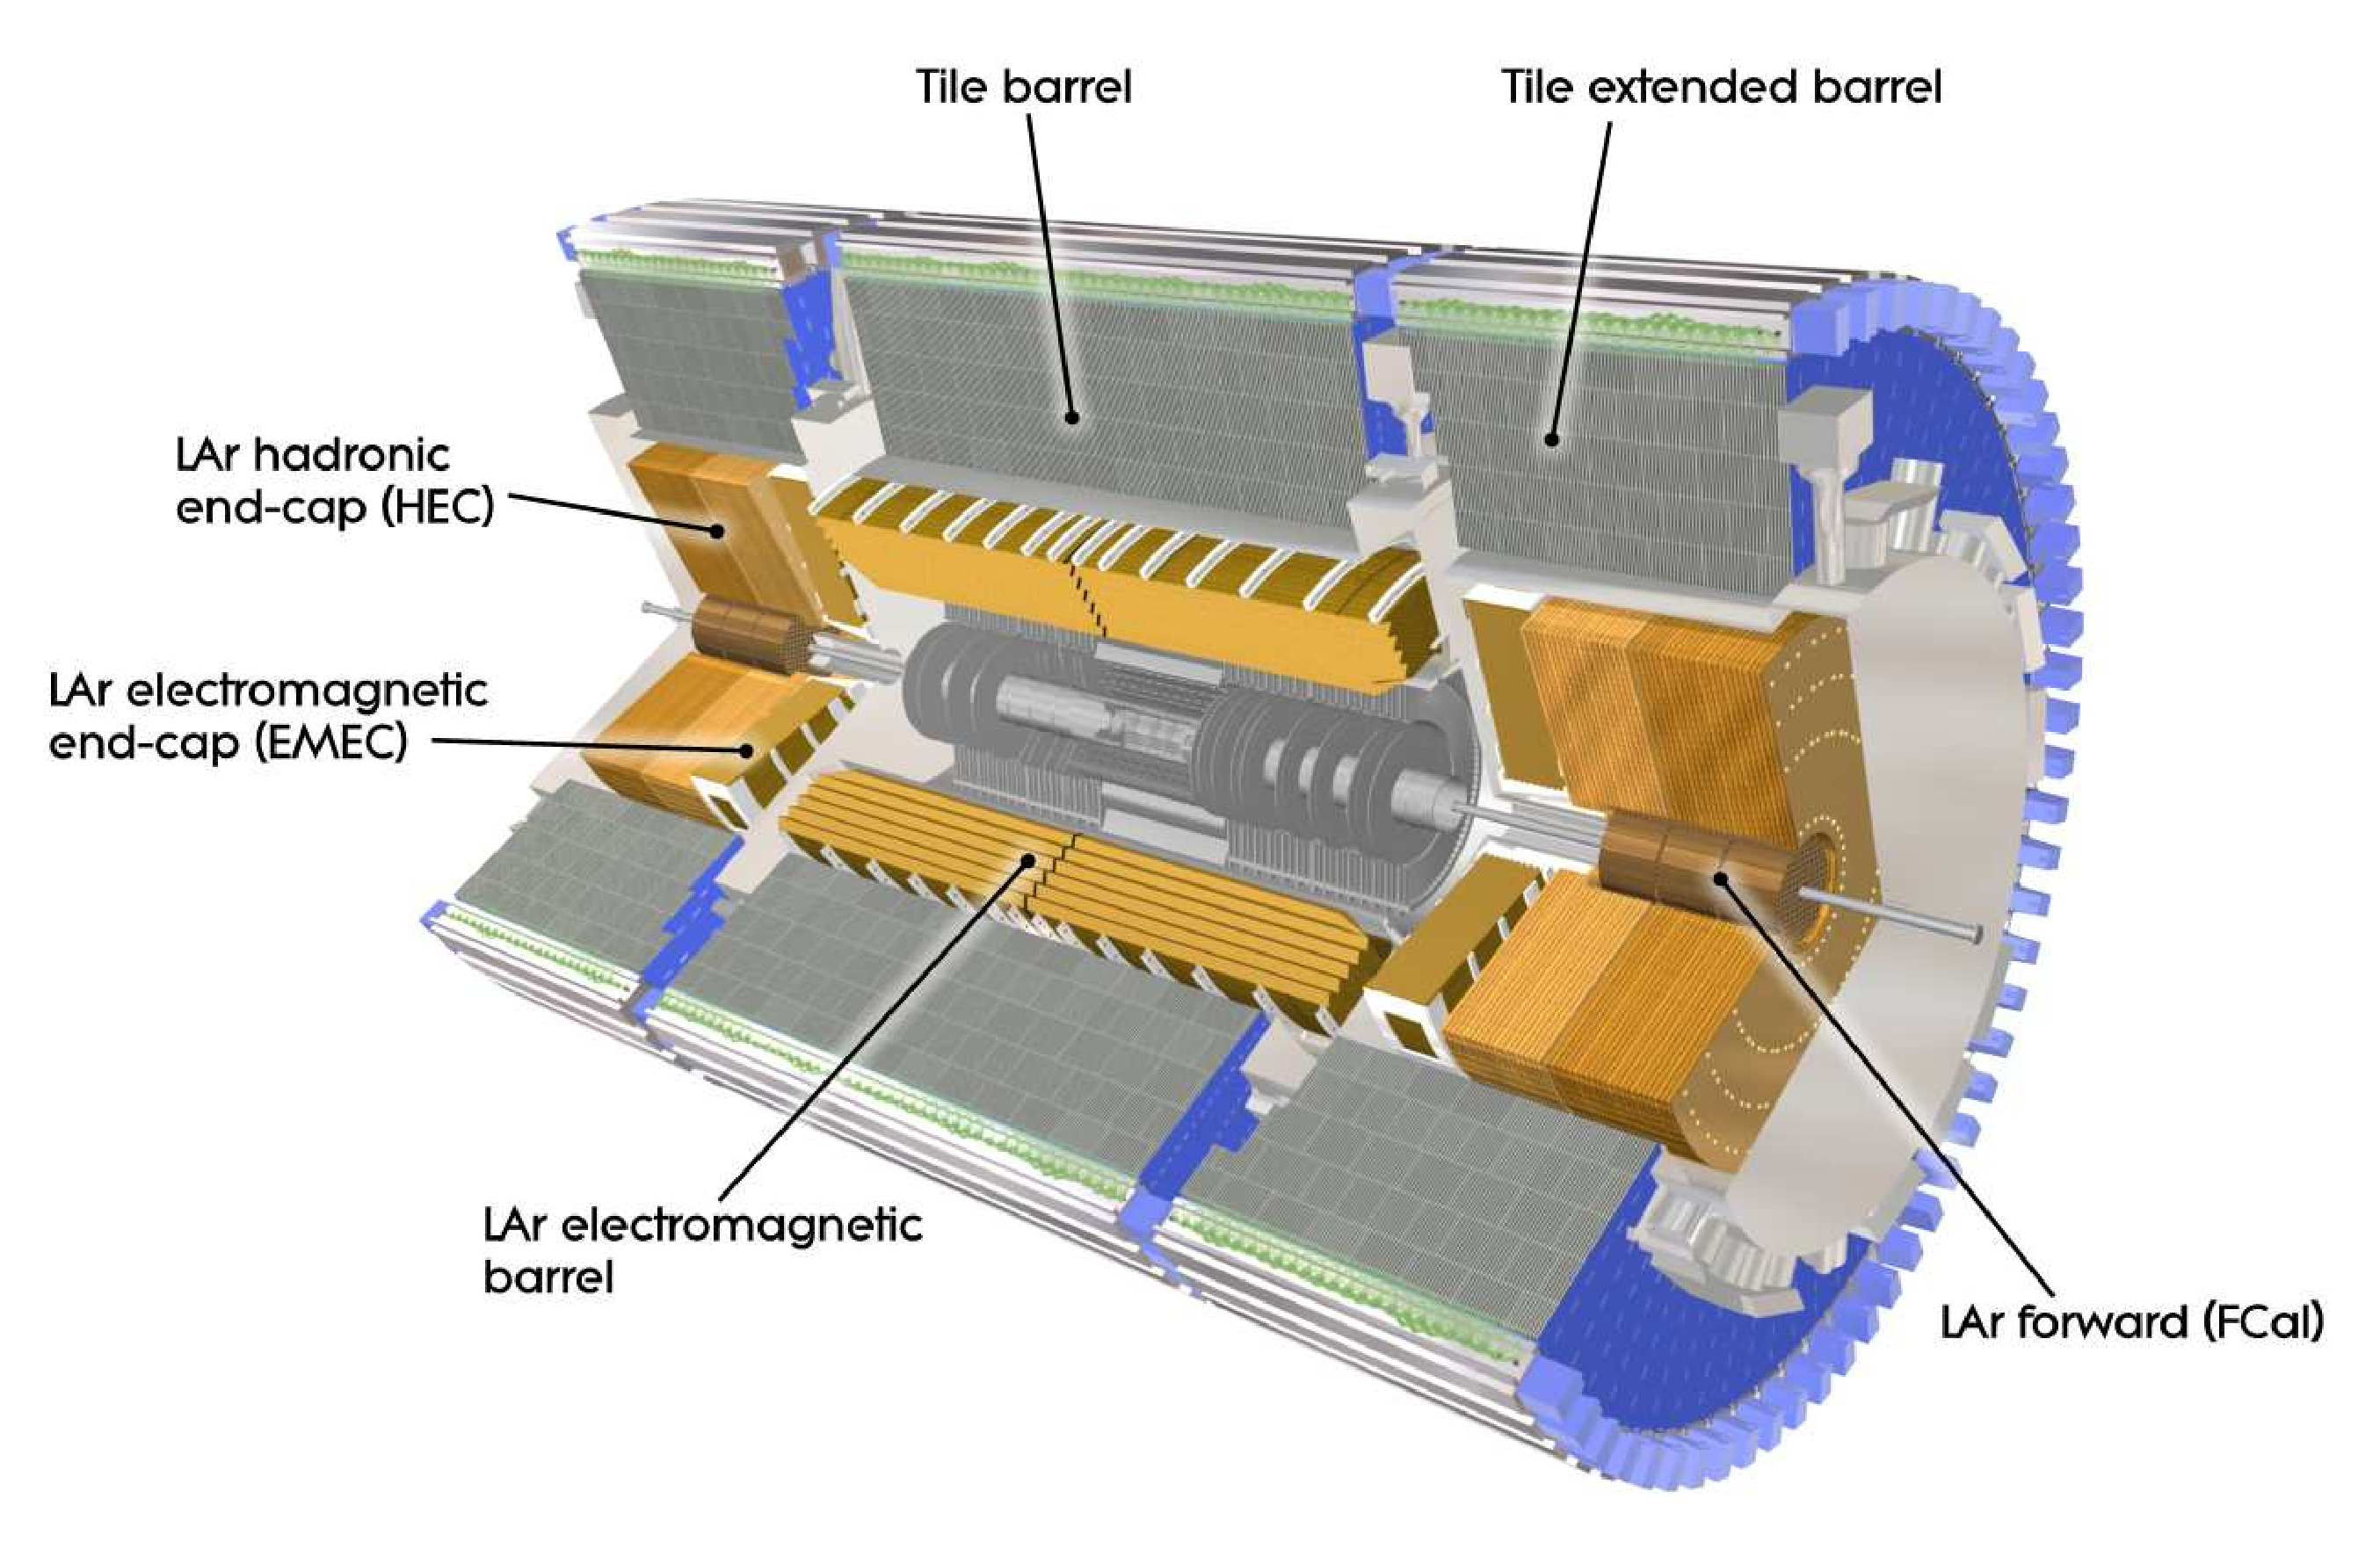
\includegraphics[width=0.8\textwidth]{figures/calorimeters.pdf} %
	\caption{The ATLAS calorimeter system. Figure taken from Ref.~\cite{Aad:2008zzm}.}	
	\label{fig:calorimeters}
\end{figure}

The ATLAS calorimeter system ~\cite{Aad:2008zzm} is the main system used for the present analysis, a picture of this system is shown in Fig.~\ref{fig:calorimeters}. The calorimeters are of sampling and non-compensating nature with a pseudorapidity coverage of $|\eta|<4.9$. The non-compensating nature gives a different response on the EM and hadronic scales, and this is corrected in the calibration procedure. A sampling calorimeter is one where two distinctly different materials are chosen, one to produce a particle shower, and the other to measure the deposited energy. 

There are two different sampling technologies used in the ATLAS calorimeter system. One technology is where liquid argon (LAr) is interspaced with lead, which acts as the absorber material. This is used in all of the ATLAS EM systems - the electromagnetic barrel (EMB), electromagnetic end-cap (EMEC), forward calorimeter (FCal), as well as the hadronic end-cap (HEC). Shower development starts in the absorber, and due to moving electrons and ions from ionization in the active material (LAr), a signal can be read out from induced charge on copper electrodes. The LAr gap is subject to a high voltage electric field in order to direct the ionized electrons and ions to the electrodes in a predictable way. The second technology, used in the hadronic tile calorimeters (TileCal), uses absorber material interspaced with plastic scintillator. The readout is different from the LAr case since scintillation light converted by wavelength shifting fibers and transported to photomultipliers instead of reading induced charge from ionization in LAr.

\subsubsection{EM Calorimeters}
\begin{figure}[ht]
	\centerline{
		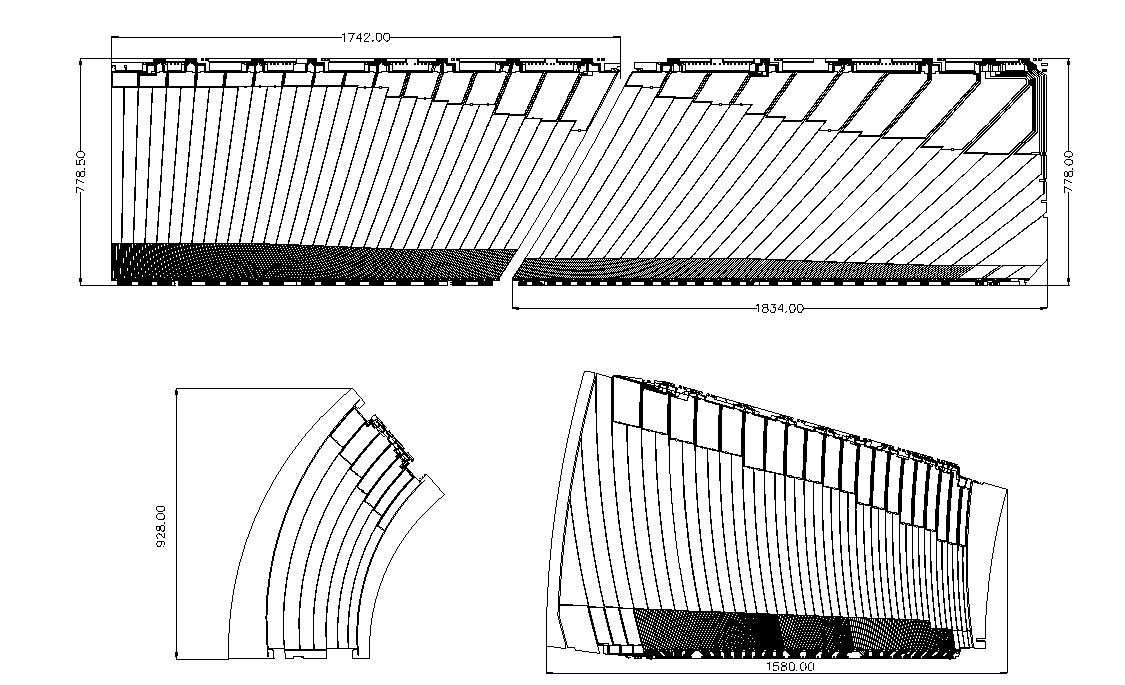
\includegraphics[width=0.7\textwidth]{figures/emmodules.pdf} 
	}
	\caption{Layouts of a barrel EM module (top), inner end-cap wheel (bottom left), and outer end-cap wheel (bottom right). Figure taken from Ref.~\cite{Aad:2008zzm}.  }
	\label{fig:emmodules}
\end{figure}

\begin{figure}[ht]
	\centerline{
		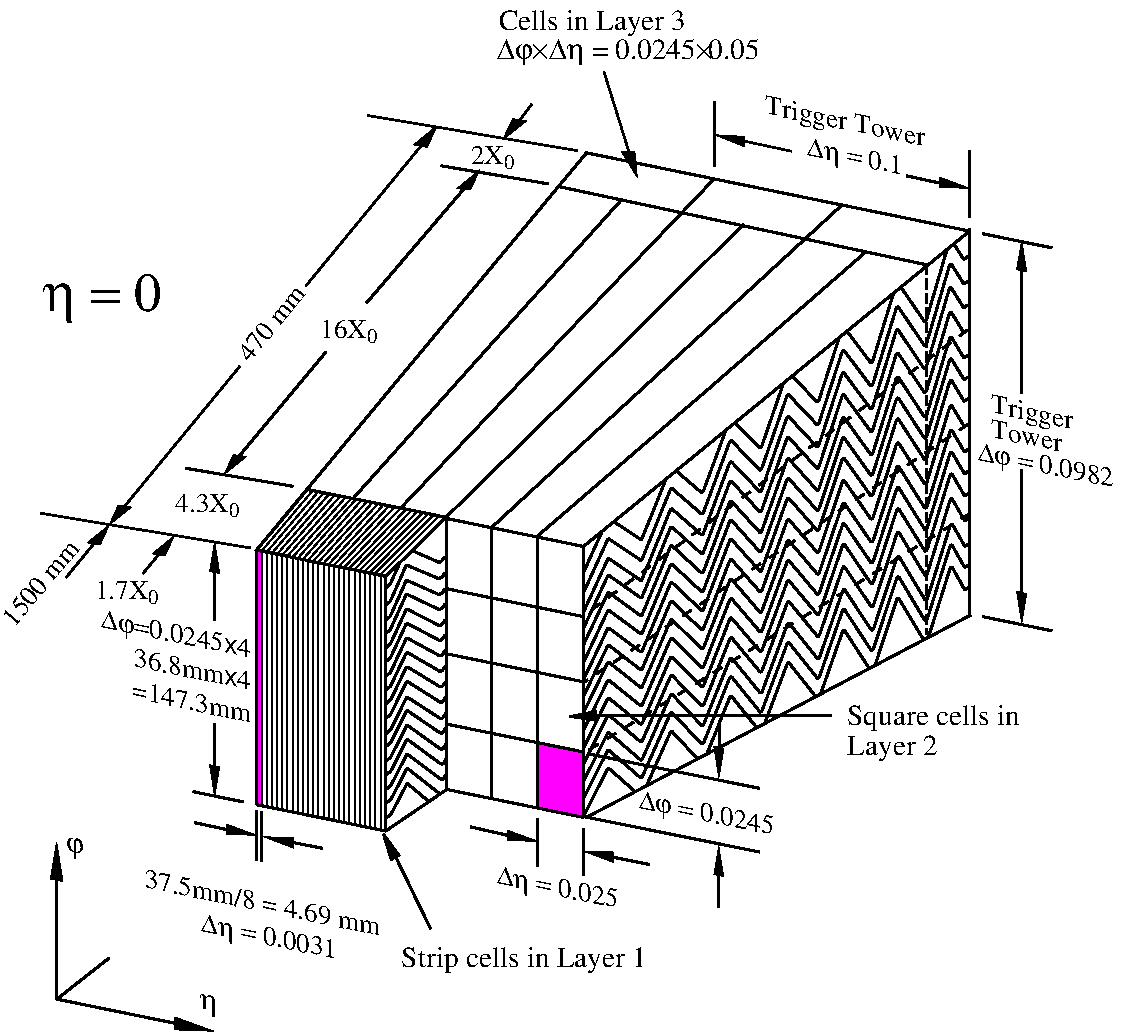
\includegraphics[width=0.7\textwidth]{figures/barrel_module.pdf} 
	}
	\caption{Sketch of a barrel EM module showing the different layers and their respective granularities. Radiation length ($X_{0}$) is the average distance an electron must travel through a given material to reduce its energy to $1/e$ of its initial energy. Trigger towers are sets of cells (strip or square) from which analog signals are summed for input to the L1 trigger. Figure taken from Ref.~\cite{Aad:2008zzm}.  }
	\label{fig:barrelemmodule}
\end{figure}

The ATLAS LAr electromagnetic calorimeter as chosen to have have an accordion geometry to minimize capacitance in the detecting elements. It is split into a barrel part covering $|\eta|<1.475$, and two end-caps covering $1.375<|\eta|<3.2$. The accordion design allows modules to have multiple layers in depth, with varying granularity ($\Deta \times \Dphi$). Layouts of segments from the barrel and end-cap EM calorimeters are shown in Fig.~\ref{fig:emmodules}. A detailed sketch of a barrel EM module and its constituent layers is shown in Fig.~\ref{fig:barrelemmodule}. All components are placed into cryostats at a temperature of approximately $86^{\circ}$ K~\cite{Bremer:449276}.  The design and size of the EM calorimeter provides a total thickness of at least 22 radiation lengths (\radlen). One \radlen\ represents the average distance an electron must travel through a material to reduce its energy to $1/e$ of its initial energy~\cite{Fabjan:2003aq}. The cumulative thickness of the calorimeter system can be seen as a function of pseudorapidity in Fig.~\ref{fig:radiationlengths}. All EM calorimeter systems were designed and tested to have an energy resolution of $\sigma(E_{T})/E_{T}=10\%/\sqrt{E_{T}}\bigoplus0.7\%$.

\begin{figure}[ht]
	\centerline{
		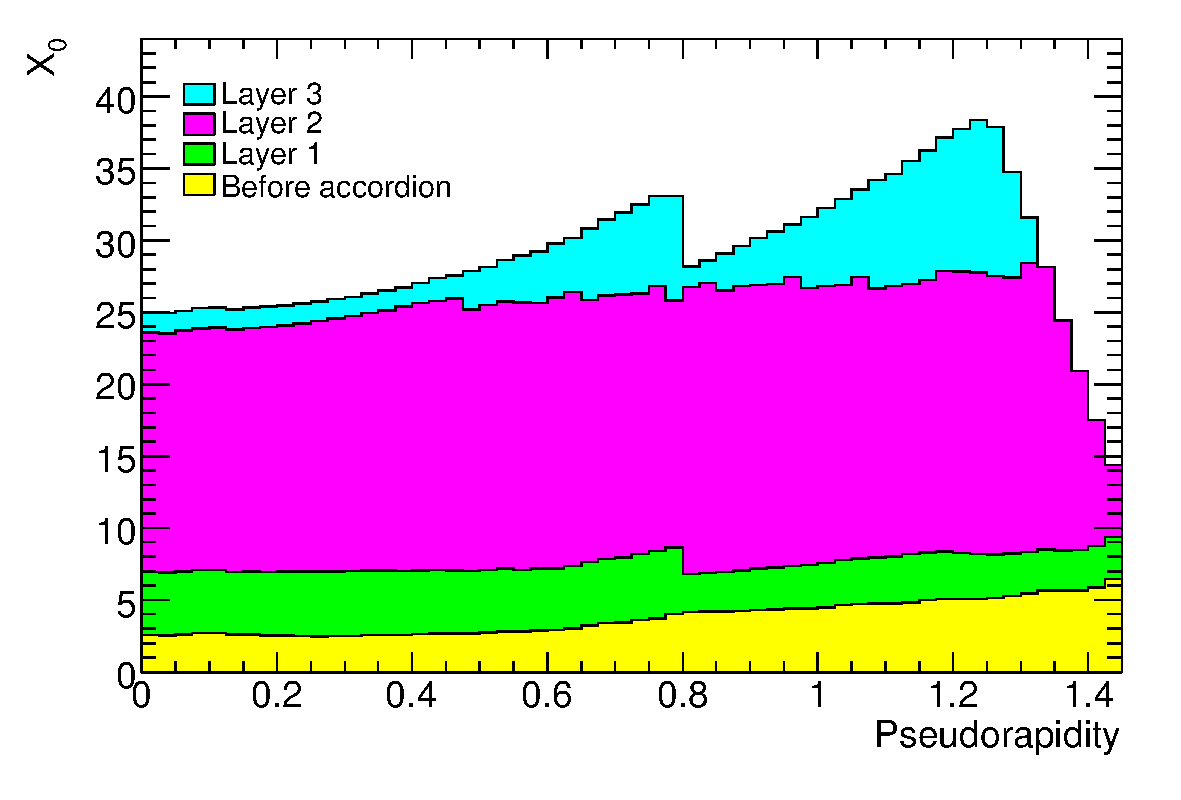
\includegraphics[width=0.49\textwidth]{figures/radiation_lengths_1.pdf} 
		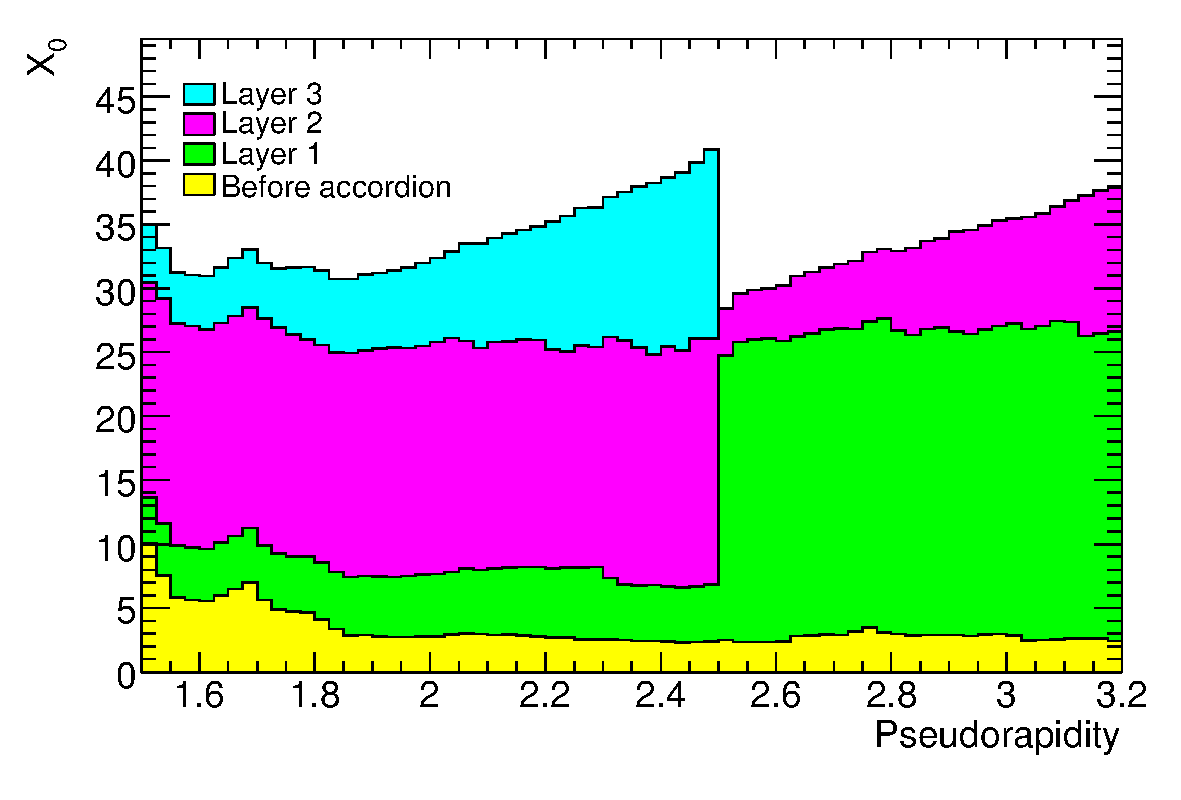
\includegraphics[width=0.49\textwidth]{figures/radiation_lengths_2.pdf} 
	}
	\caption{Cumulative thickness, in units of radiation length \radlen\ and as a function of $|\eta|$, in front of (yellow distribution) and in the electromagnetic calorimeters. Shown separately are the amounts of radiation in the various layers of the barrel (left) and end-cap (right) EM calorimeters. Figure taken from Ref.~\cite{Aad:2008zzm}. }
	\label{fig:radiationlengths}
\end{figure}

A typical pulse in the LAr calorimeter originates from ionization electrons in the LAr gap. An electric field inside the gap collects the electrons and an ionization pulse is then read out and shaped. An ionization pulse is triangular in shape has a width of $\sim$450 ns~\cite{Nikiforou:2013nba}, as can be seen in Fig.~\ref{fig:larsignal}. The final pulse that is digitized has a width between 450 and 600 ns after shaping. This corresponds to roughly 18 to 24 LHC bunch crossings. During this time, there could be contributions from out-of-time events (pile-up), and various techniques such as optimal filtering~\cite{OliveiraDamazio:1630826} have been developed to minimize contributions from pile-up.

\begin{figure}[ht]
	\centerline{
		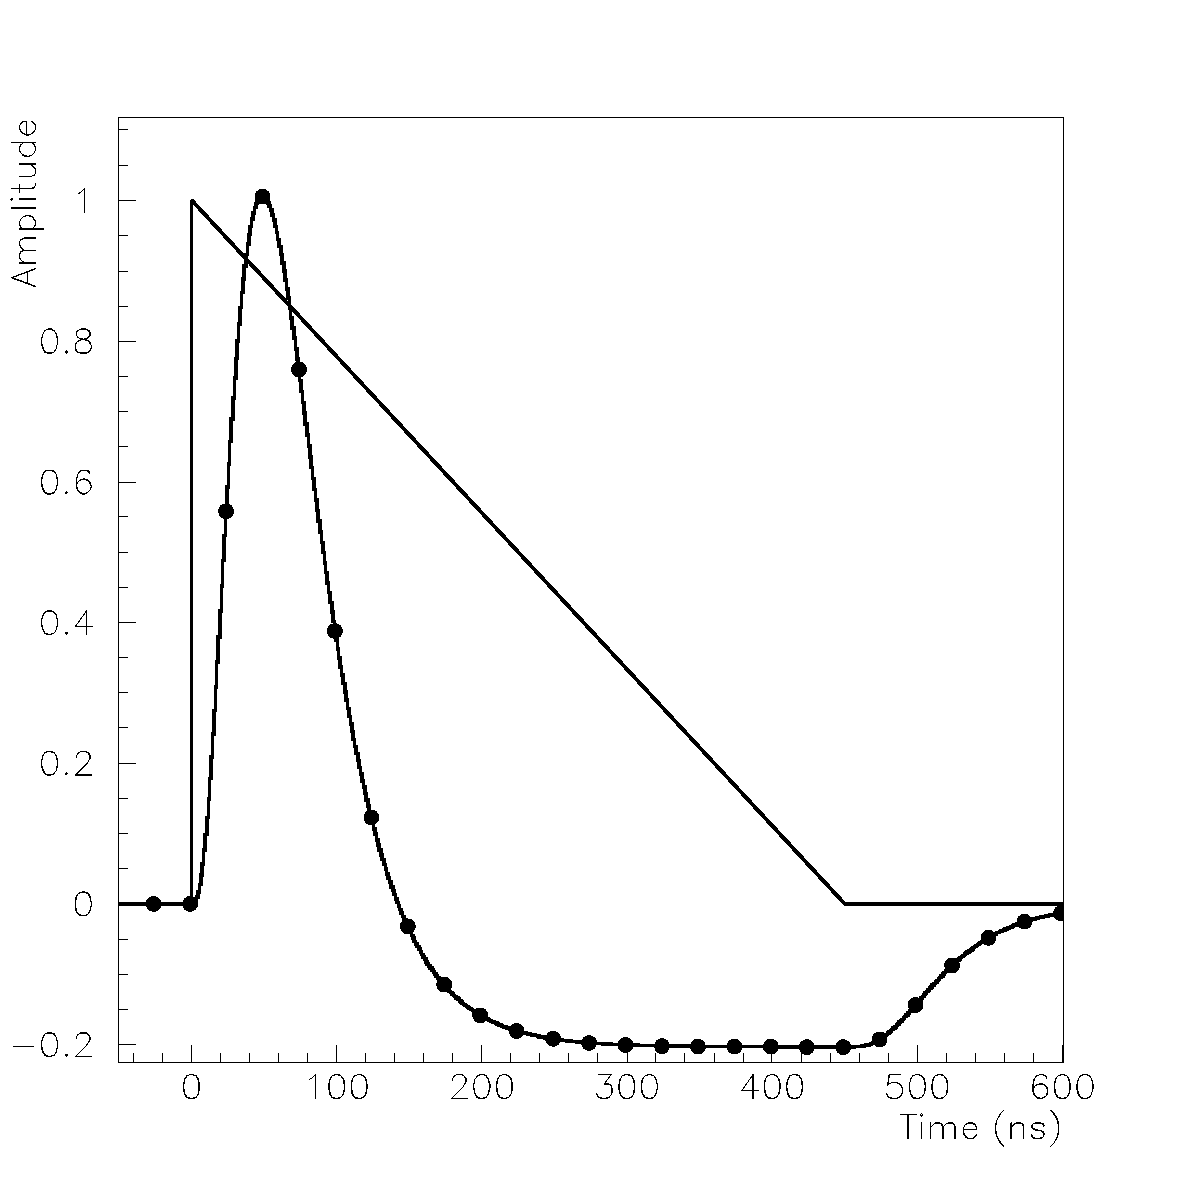
\includegraphics[width=0.5\textwidth]{figures/lar_signal.pdf} 
	}
	\caption{Amplitude versus time plot of a LAr calorimeter pulse before shaping (triangular). The shaped pulse is sampled every 25 ns, as indicated by the periodic points. The sampling frequency corresponds to the LHC bunch crossing frequency of 25 ns. Figure taken from Ref.~\cite{Aad:2008zzm}.}
	\label{fig:larsignal}
\end{figure}

\subsubsection{EM Barrel Calorimeter}
The EM barrel, covering $|\eta|<1.475$, consists of two half-barrels, each 3.2 meters long and weighing 57 tons. It has an inner and outer diameter of 2.8 m and 4.0 m, respectively. The calorimeter is comprised of three layers, with a thickness of at least 22 \radlen\, increasing to from 22 to 30 \radlen\ in the interval $0<|\eta|<0.8$, and from 24 to 33 \radlen\ in the interval $0.8<|\eta|<1.3$, as seen in Fig.~\ref{fig:radiationlengths}. In front of these three layers is a LAr presampler which is intended to recover energy lost to material in front of the EMCal. The granularity of the EM barrel calorimeter's first layer is $\Deta\times\Dphi=0.025\times0.025$ in order to be able to perform shower shape measurements and to distinguish pairs of $\gamma$ from $\pi^{0}$ decays with pairs of $\gamma$ from $H$ decay. The granularity of the presampler is $\Deta\times\Dphi=0.025\times0.1$. 


\subsubsection{EM End-cap Calorimeter}
The EM end-cap calorimeter, covering $1.375<|\eta|<3.2$, consists of two wheels on each side of the EM barrel calorimeter, each 63 cm thick, with a weight of 27 tons. Each wheel of the EM end-cap calorimeter consists of 32 identical azimuthal sectors. Similar to the EM barrel calorimeter, the barrel end-cap calorimeter consists of three layers. It has a total thickness of at least 24 \radlen\, increasing from 24 to 38 \radlen\ on the outer wheel ($1.475<|\eta|<2.5$), and from 26 to 36 \radlen\ on the inner wheel ($2.5<|\eta|<3.2$). Similar to the EM barrel calorimeter, the granularity of the first layer is $\Deta\times\Dphi=0.025\times0.025$ and the granularity of the presampler is $\Deta\times\Dphi=0.025\times0.1$.

\subsubsection{Hadronic Calorimeters}

\begin{figure}
	\centering
	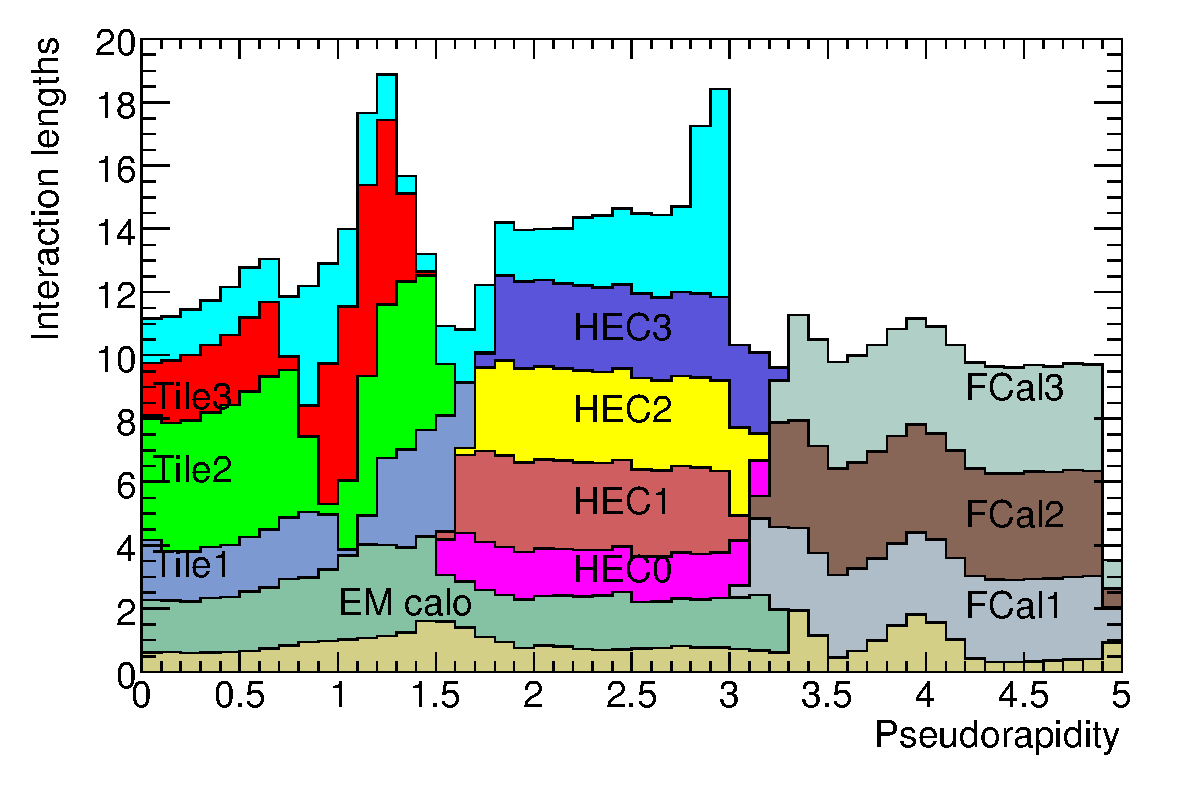
\includegraphics[width=0.7\textwidth]{figures/interaction_lengths.pdf} %
	\caption{Cumulative thickness, units of interaction length (\intlen) as a function $\eta$, in front of the EM calorimeters, in the EM calorimeters themselves, in the hadronic calorimeters, and the total amount after all calorimeters. Figure taken from Ref.~\cite{Aad:2008zzm}.}	
	\label{fig:interactionlengths}
\end{figure}

The hadronic calorimeters surround the EM calorimeters and are designed to measure the energy deposited from hadrons and hadronic showers that passed through the EM calorimeters. Characteristic distance for hadronic calorimeters is described by the nuclear interaction length \intlen, which is the hadronic equivalent to a radiation length.  For the EM calorimeter system, \intlen\ is small, requiring hadronic calorimeters to have sufficiently larger thicknesses in order to fully contain hadronic showers. The hadronic calorimeter is composed of the Tile barrel calorimeter with a coverage $|\eta|<0.8$, the Tile extended barrel with a coverage $0.8<|\eta|<1.7$, and the HEC with a coverage $1.5<|\eta|<3.2$. Both Tile systems use steel as an absorber, with scintillator as the active material. The particle shower begins in the absorber, and scintillation light then gets transported through the wavelength shifting fiber into photomultiplier tubes where the signal is read out. The HEC is based on the same LAr technology used in the EM calorimeters, but uses copper, instead of lead, for the absorber material. Total interaction lengths of the ATLAS calorimeter system as a function of pseudorapidity are summarized in Fig.~\ref{fig:interactionlengths}. Both TileCal and HEC calorimeters have an energy resolution of $\sigma(E_{T})/E_{T}=50\%/\sqrt{E_{T}}\bigoplus3\%$. 

\subsubsection{Tile Barrel and Extended Barrel Calorimeters}
The Tile barrel and extended barrel calorimeters cover $|\eta|<0.8$ and $0.8<|\eta|<1.7$ respectively. The tile barrel calorimeter is 5.8 m long, the two tile extended barrels are each 2.6 m in length. Both the tile barrel and extended barrel calorimeters have an inner and outer diameter of 2.28 m and 4.25 m, respectively. They is composed of three layers with granularity of $\Deta\times\Dphi=0.1\times0.1$ for the first two layers, and the outermost layer with granularity $\Deta\times\Dphi=0.2\times0.1$. Each barrel consists of 64 modules roughly $\Dphi=0.1$ in size. A schematic showing a TileCal module is shown in Fig.~\ref{fig:tilecalmodule}.

\begin{figure}
	\centering
	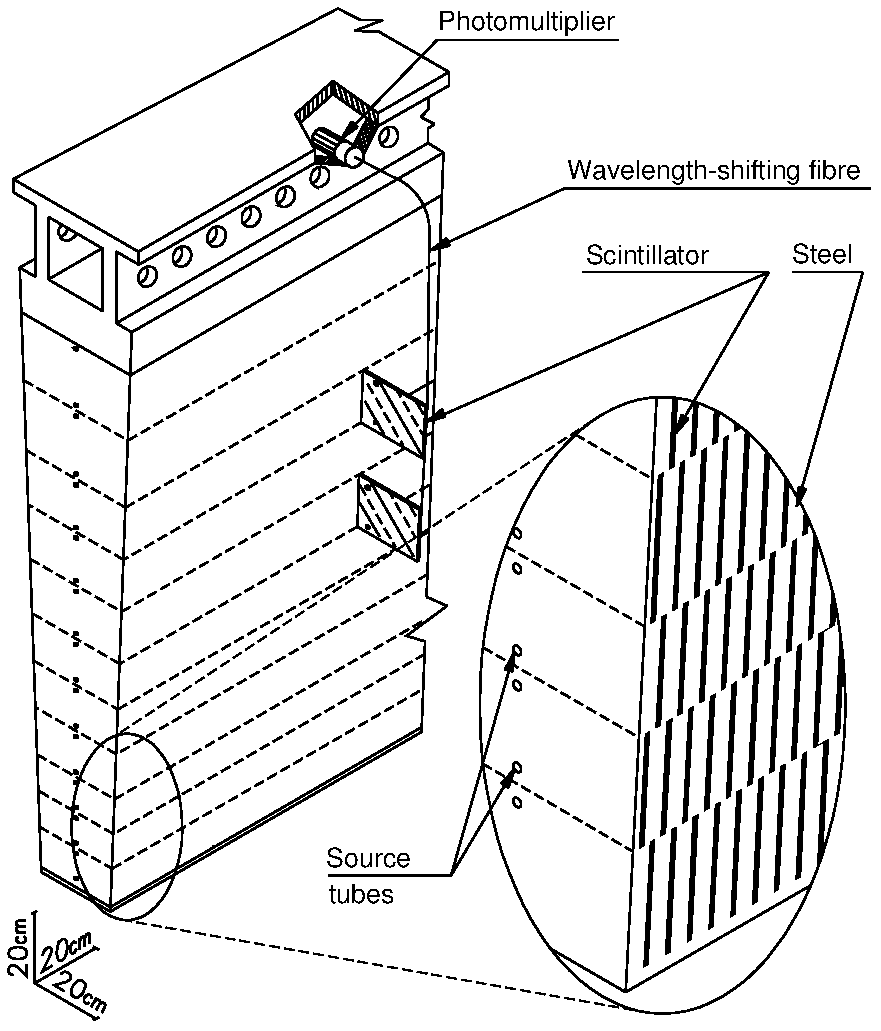
\includegraphics[width=0.5\textwidth]{figures/tile_1.pdf} %
	\caption{ Schematic of a TileCal module, showing absorber material interspace with scintillator. Figure taken from Ref.~\cite{Aad:2008zzm}.}	
	\label{fig:tilecalmodule}
\end{figure}

\subsubsection{LAr Hadronic End-Cap Calorimeter}
The HEC calorimter is based the LAr technology used in the EM calorimter systems. The absorber material is copper, and the active material is LAr. The HEC covers a pseudorapidity region of $1.5<|\eta|<3.2$. The two barrels of the HEC each contain 32 modules symmetric in azimuth, with an outer radius of 2030 mm. The first two layers of the HEC have a granularity $\Deta\times\Dphi=0.1\times0.1$, while the last layer has a courser granularity of $\Deta\times\Dphi=0.2\times0.2$.

\subsubsection{Forward Calorimeter}

\begin{figure}
	\centering
	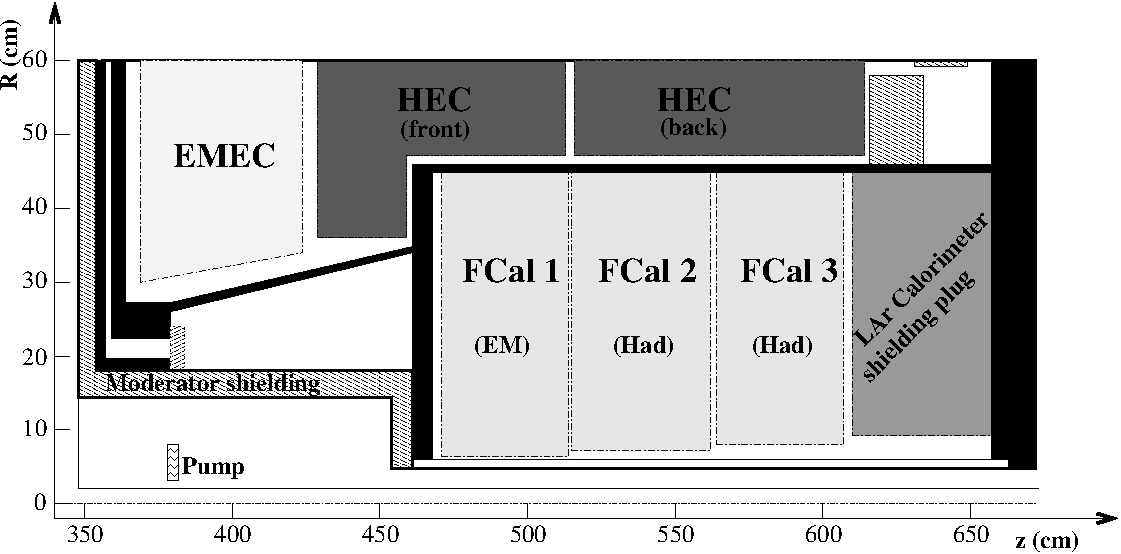
\includegraphics[width=0.75\textwidth]{figures/fcal_1.pdf} %
	\caption{ Diagram showing the three modules of the FCal. Shown in the $y-z$ plane, with the beam going in the $z$ direction. The FCal is the most forward calorimeter in ATLAS, covering a pseudorapidity interval $3.2<|\eta|<4.9$. Figure taken from Ref.~\cite{Aad:2008zzm}.}	
	\label{fig:fcalmodules}
\end{figure}

The forward calorimeter is an important sub-system in the present analysis due to its forward pseudorapidity coverage. The calorimeter is comprised of two halves located on either side of the ATLAS detector IP, surrounded by the HEC. It covers a pseudorapidity range of $3.2<|\eta|<4.9$, and has a granularity of $\Deta\times\Dphi=0.2\times0.2$. While the other EM calorimeter systems use an accordion design, the forward calorimeter has electrodes oriented parallel to the beamline (z-axis) which consist of thin tubes of copper with a gap for LAr that surround rods of absorber material. These tubes are located inside the same kind of absorber material. The LAr gap is thin, about 0.25 mm in the first module, in order to increase readout time and decrease noise from ion buildup.

\begin{figure}
	\centering
	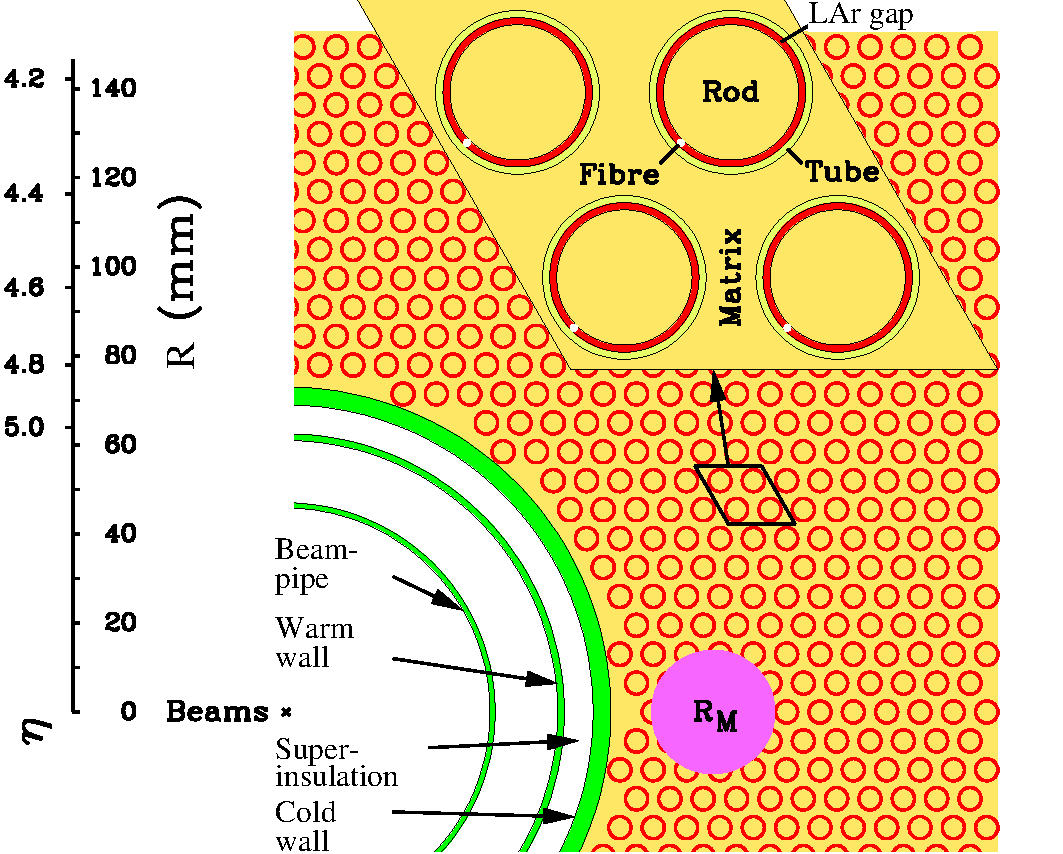
\includegraphics[width=0.575\textwidth]{figures/fcal_2.pdf} %
	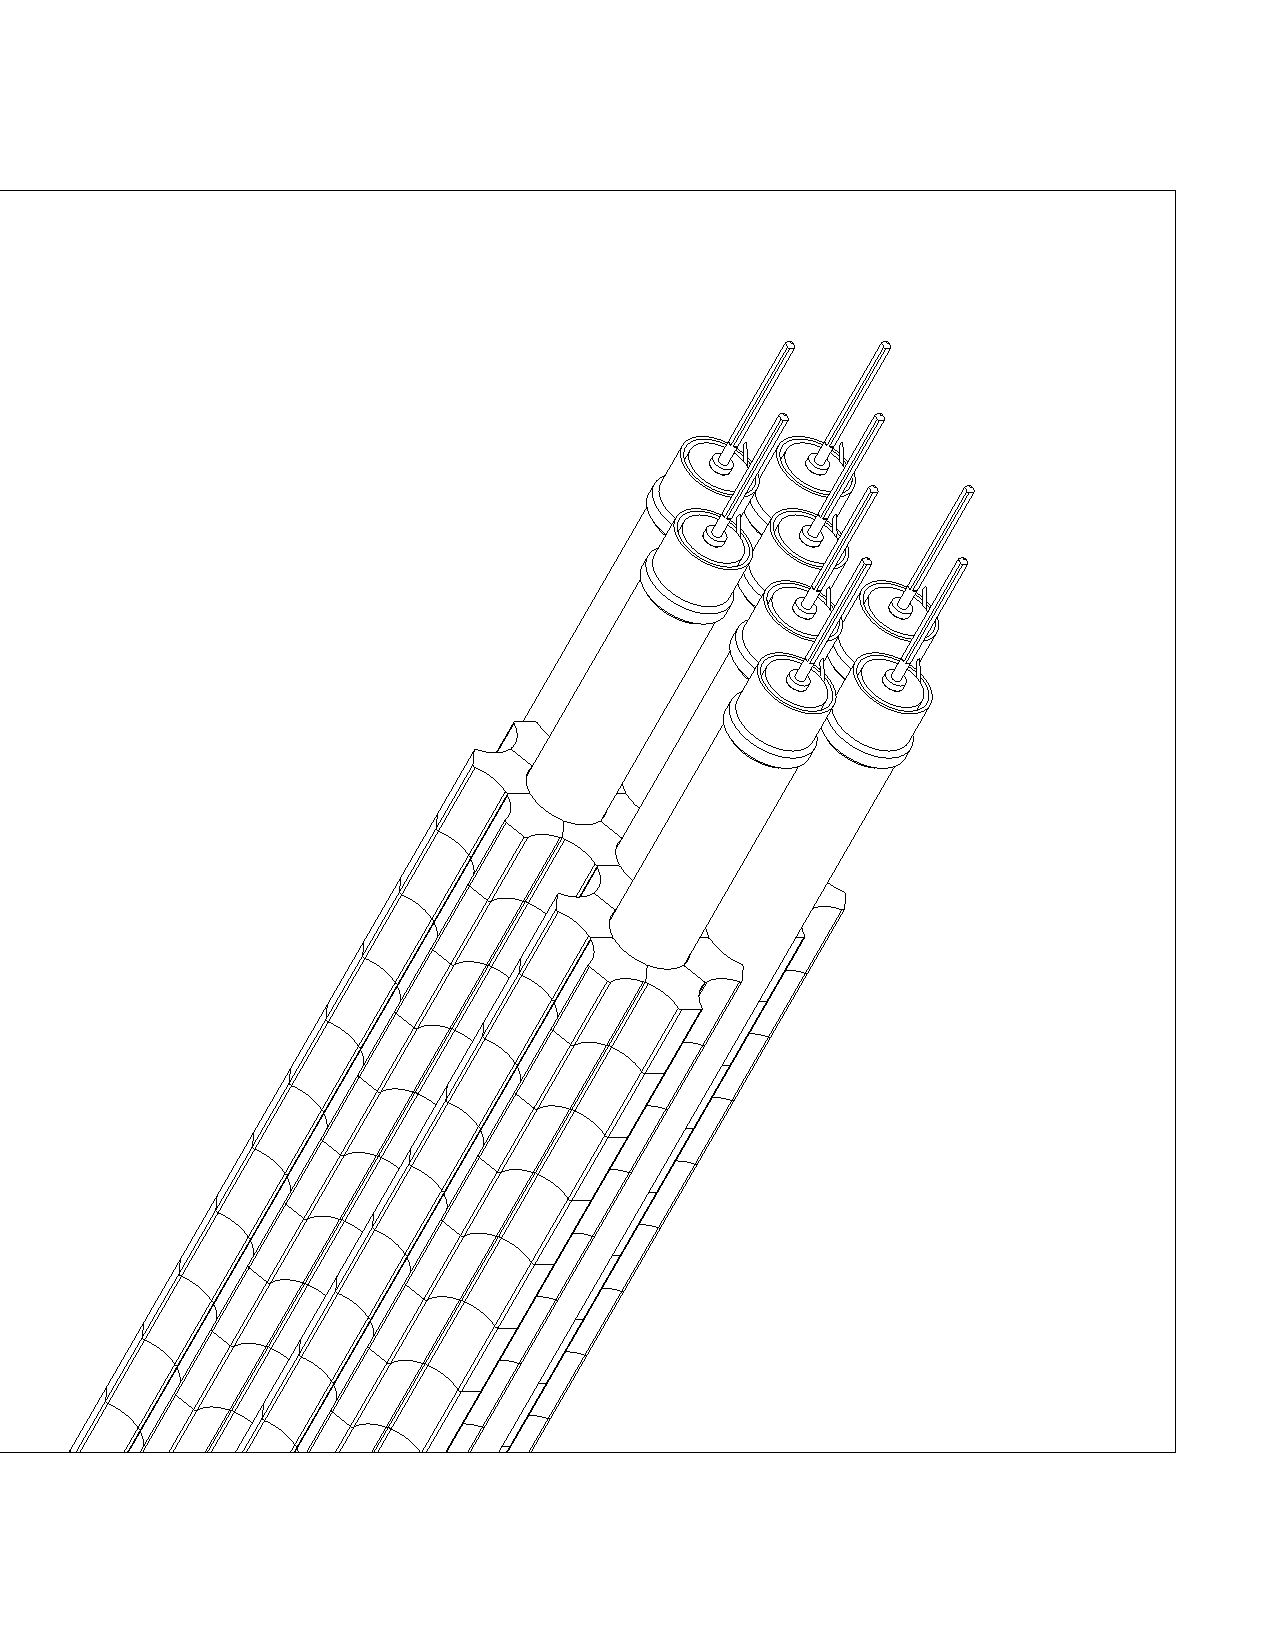
\includegraphics[width=0.375\textwidth]{figures/fcal_3.pdf} %
	\caption{ View of first FCal module (EM) as seen along the z-axis (left). Tubes of LAr inside absorber material. Shown is one Moliere radius $R_{M}$, which is the radius of a cylinder that would contain 90\% of the radiation inside a calorimeter. A schematic of the tungsten rods, enclosed in copper and a LAr gap, all surrounded by tungsten slugs (right). The design is used for the two hadronic FCal modules FCal2 and FCal3. Figures taken from Ref.~\cite{Aad:2008zzm}.}	
	\label{fig:fcalcloseup}
\end{figure}

Each FCal is composed of three modules, as shown in the $y-z$ plane in Fig.~\ref{fig:fcalmodules}. The first of three modules (FCal1) is the EM module and uses copper as the absorber. The last two hadronic modules (FCal2, FCal3) use tungsten as the absorber. FCal1 uses copper plates that are stacked one behind the other. These plates have 12,260 drilled holes to make space for the electrodes, which are rods made from absorber material coaxial to a thin surrounding LAr layer with precision, radiation-hard plastic fiber used for readout.  A schematic of first layer of the calorimeter as it appears in the $x-y$ plane, perpendicular to the beam direction, showing the tubes of LAr inside the absorber material, is shown in the left of Fig.~\ref{fig:fcalcloseup}. Signal is read out from ionized charges in the LAr that travel to electrodes which run parallel to the tubes. The hadronic modules FCal2 and FCal3 require large interaction lengths, which is why tungsten is chosen as the absorber material, rather than copper as in FCal1. The modules consist of two copper plates, 2.35 cm thick, that have many tungsten rods, coaxial to copper tubes with a LAr gap, enclosed in tungsten slugs, as shown in right of Fig.~\ref{fig:fcalcloseup}. These modules give a total of 10 \intlen\ interaction lengths. The FCal has an energy resolution of $\sigma(E_{T})/E_{T}=100\%/\sqrt{E_{T}}\bigoplus10\%$. 

\subsection{Solenoid Magnet}
The magnet system, shown in Figure~\ref{fig:magnet} has an overall dimension of 22 m in dameter and 26 m in length. It stores a total energy of 1.6 GJ and consists of a barrel solenid magnet, and toroidal magnets used by the muon system. The toroidal magnets are not used in the present analysis. The solenoid magnet, which is used by the inner detector tracker, provides a 2 T axial field which is supplied by a 7.73 kA current. NbTi is used as a conductor and is supercooled by a LAr cryostat temperatures down to 4.5 K. 


\begin{figure}
	\centerline{
		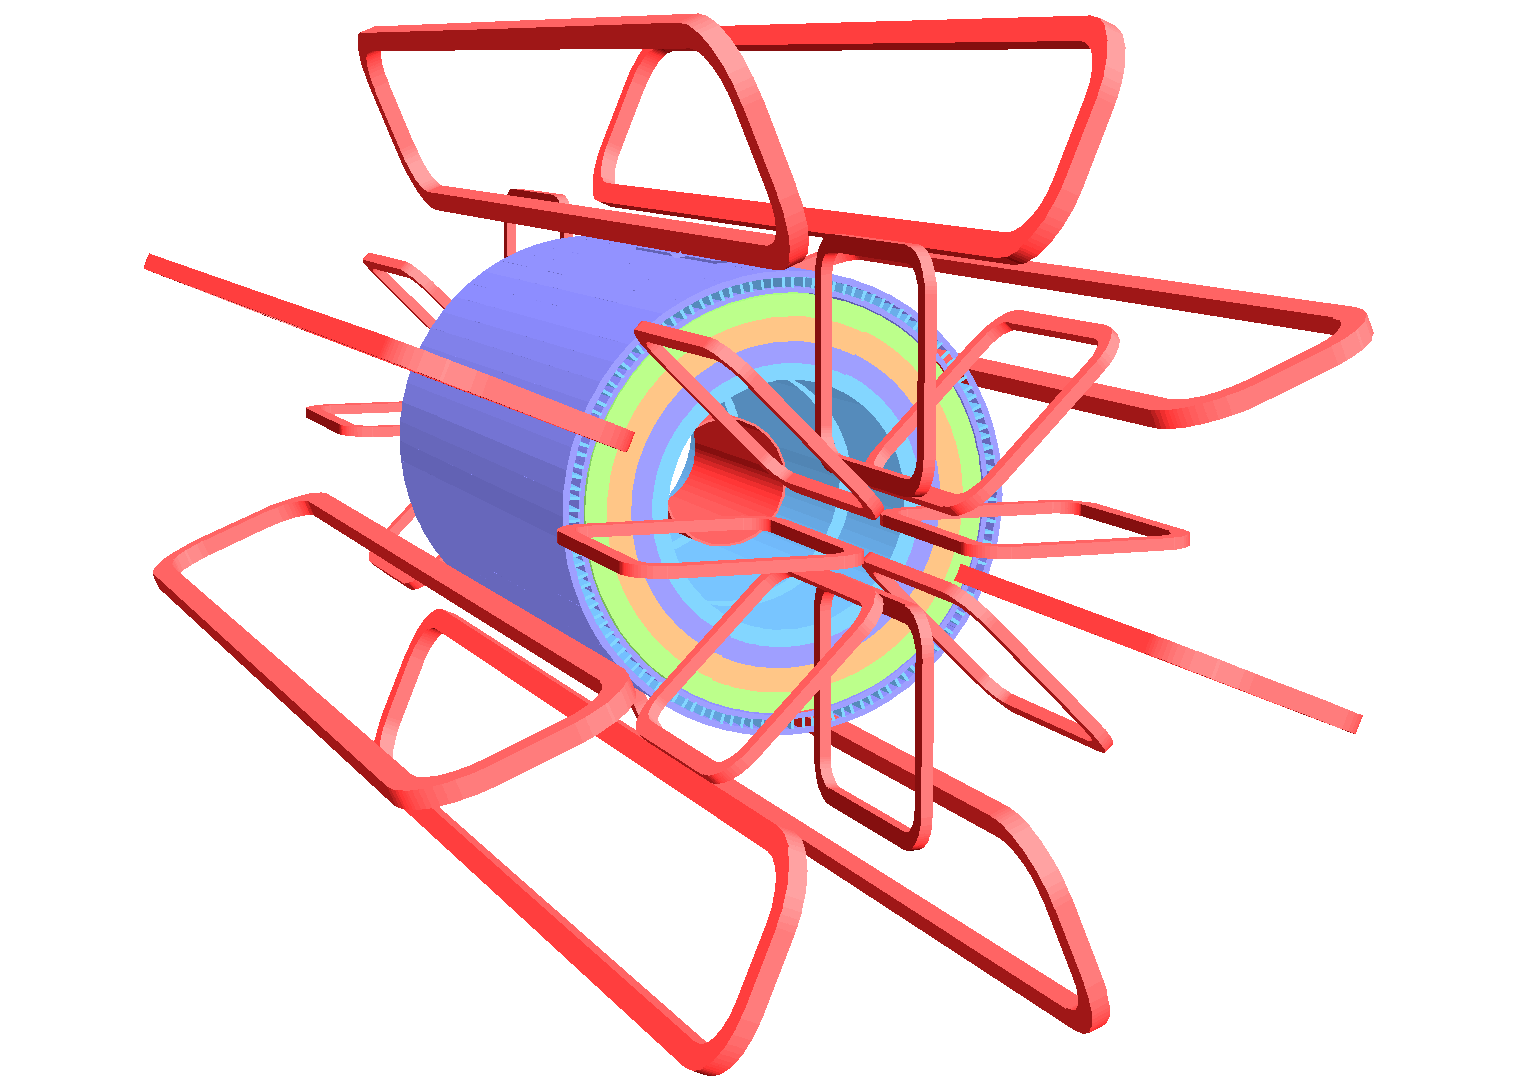
\includegraphics[width=0.52\textwidth]{figures/magnet.pdf} %
	}
	\caption{ The ATLAS magnet system. Shown is the cylindrical solenoid magnet, as well as the eight barrel toroid magnets used for muon detection. Figure taken from Ref.~\cite{Aad:2008zzm}.}	
	\label{fig:magnet}
\end{figure}

\subsection{Inner Detector}

The ATLAS Inner Detector (ID) is responsible for tracking, which is the precise determination of the position of charged particles. In an average collision there can be thousands of particles, which, in in the presence of a magnetic field, will curve. If their positions are well known and can be distinguished, the particles momentum can be calculated. The ID is designed to provide precision tracking for particles above a \pt\ threshold of 0.5 GeV, although some studies have had similar performance with particle \pt\ as low as 0.1 GeV. The ID is designed to have a transverse momentum resolution of $\sigma(\pt)/\pt=0.05\%/\sqrt{E_{T}}\bigoplus1\%$.  Tracking is a very important part of every high energy particle detector, and is usually placed closest to the interaction point of a detector. A cut-away and schematic of the ID is shown in Fig.~\ref{fig:id}. The detector sits inside the 2T magnetic field produced by the solenoid. The ID has a rapidity coverage of $|\eta|<2.5$ and has an outer radius of 1.15 m. There are there main subsystems that comprise the ID, listed outwards from the beam pipe: the pixel detectors, the semiconductor tracker (SCT), and the transitional radiation tracker (TRT).

\begin{figure}
	\centerline{
		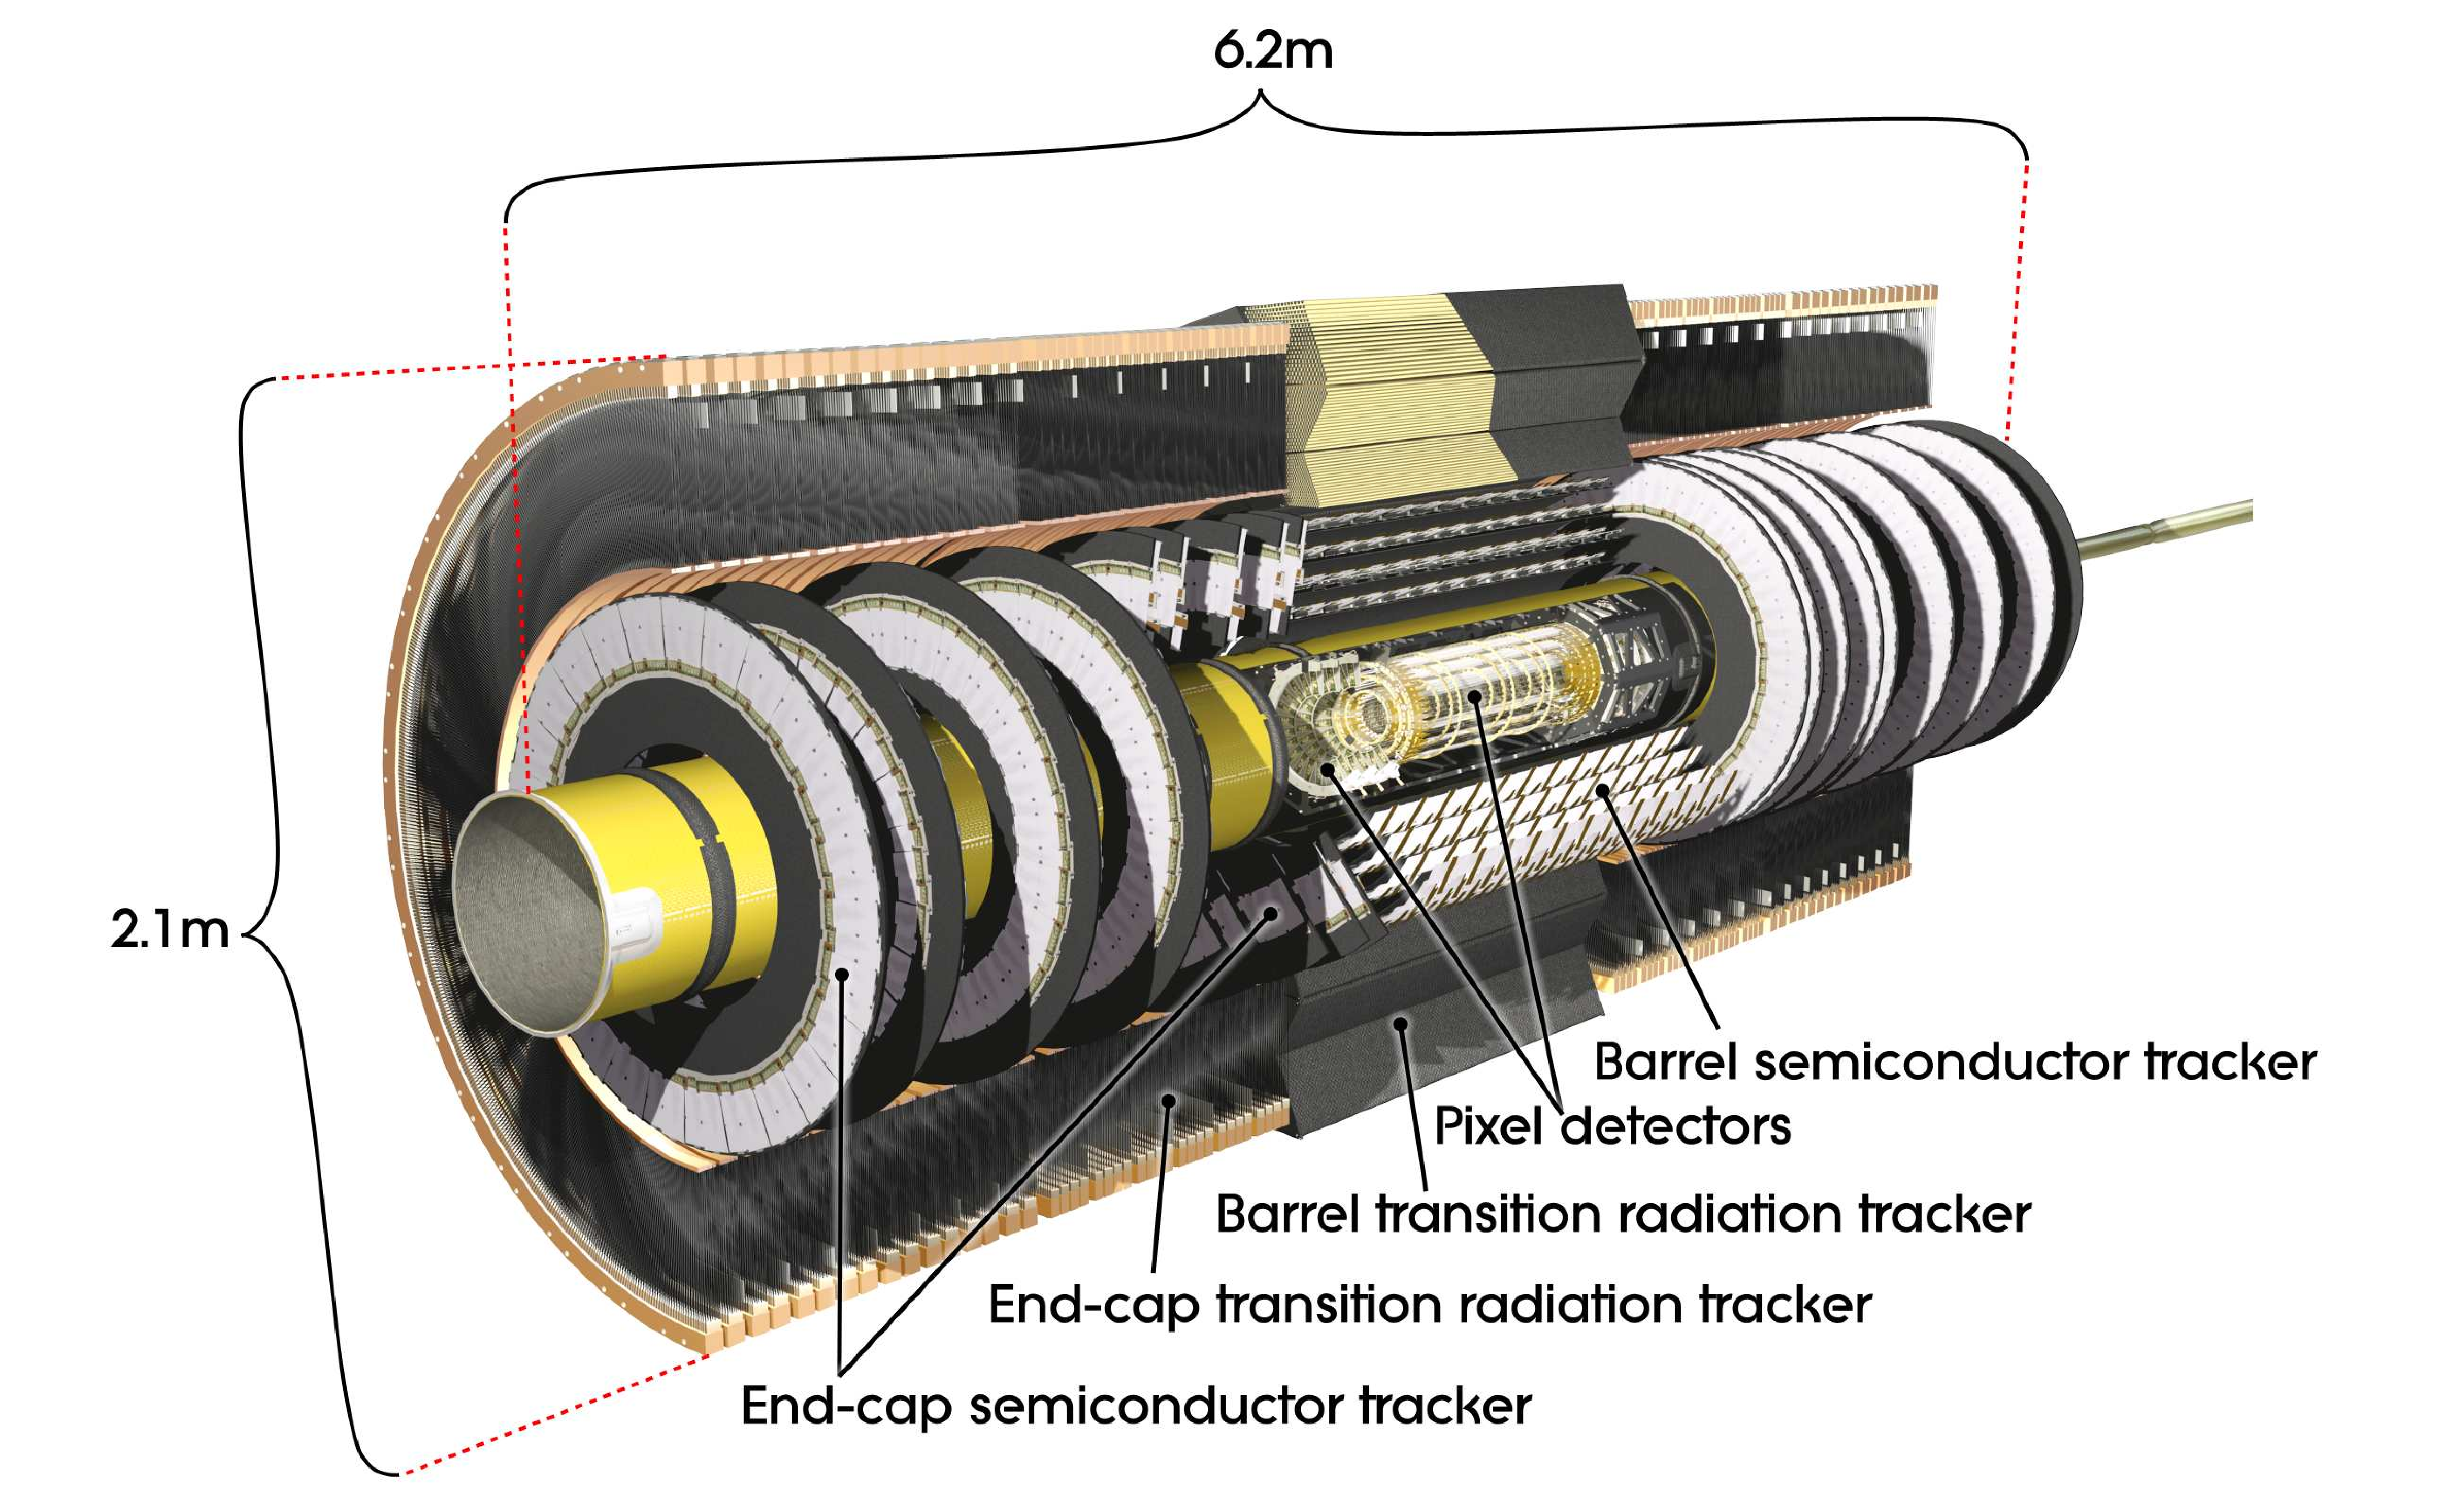
\includegraphics[width=0.52\textwidth]{figures/id.pdf} %
		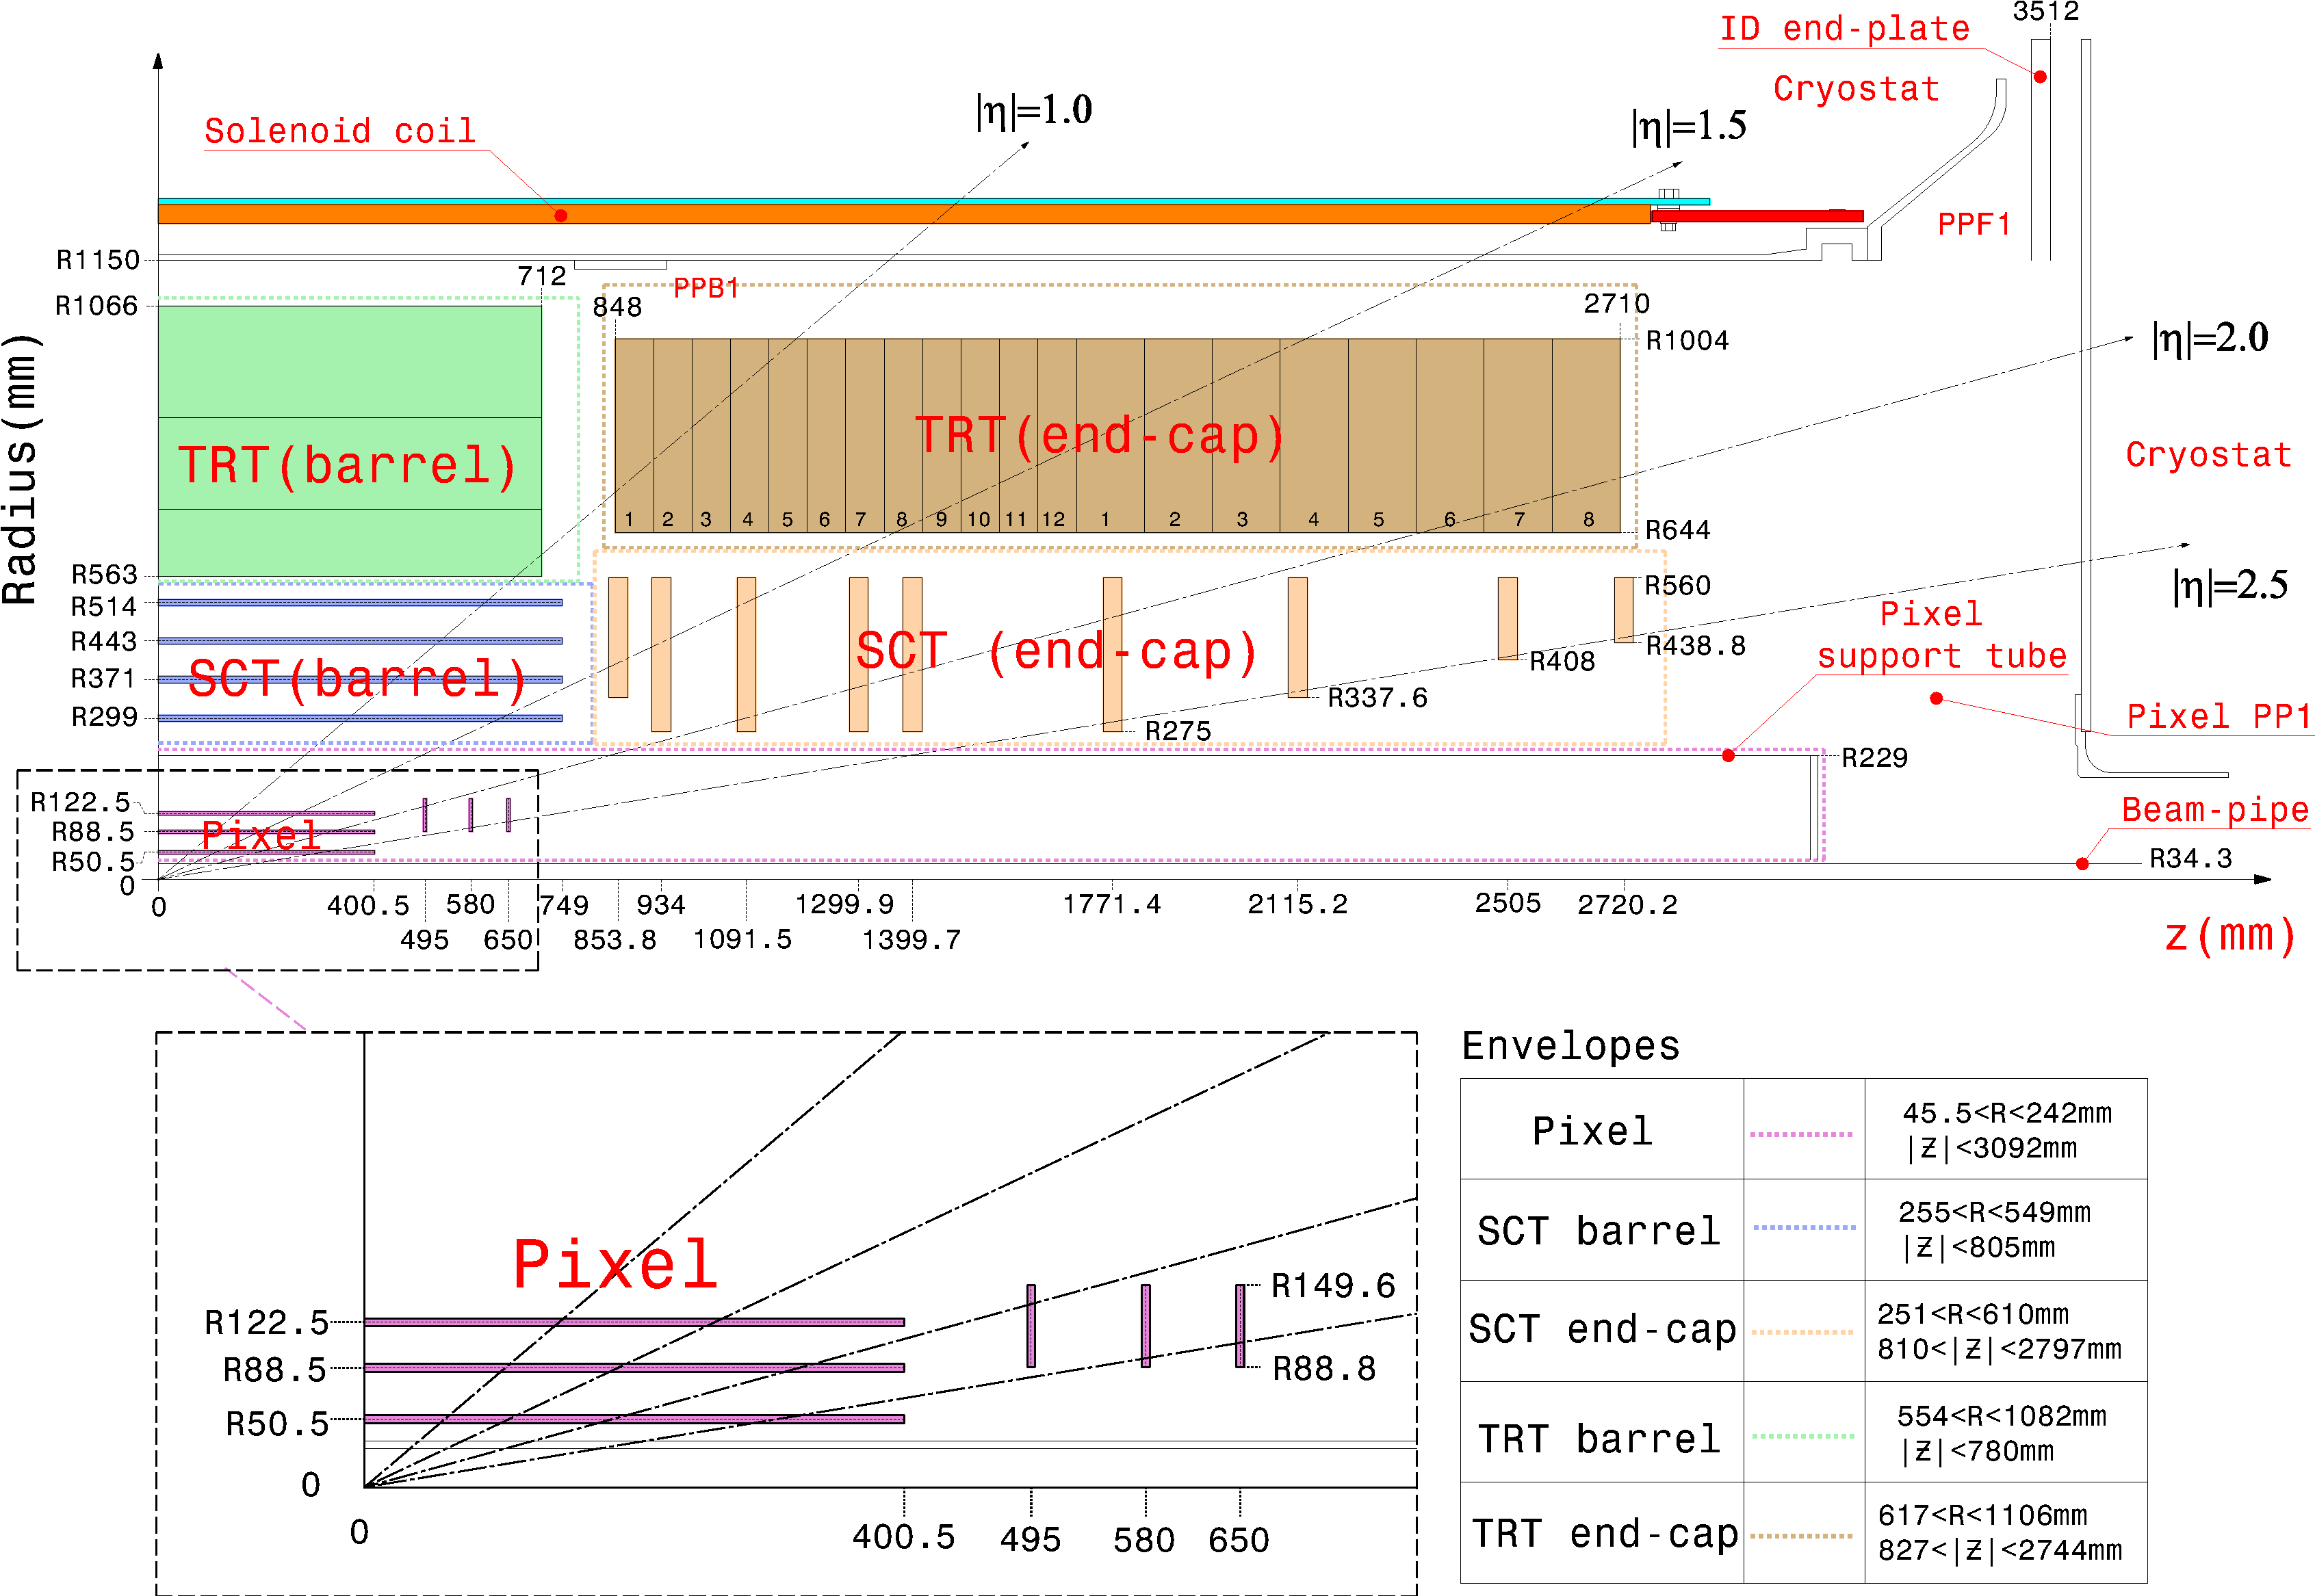
\includegraphics[width=0.52\textwidth]{figures/id_schematic.pdf} %
	}
	\caption{ Cut-away picture (left) and schematic (right) of the ATLAS Inner Detector. Figures taken from Ref.~\cite{Aad:2008zzm}.}	
	\label{fig:id}
\end{figure}

The pixel layer has the highest granularity out of the ATLAS tracking subsystems. There is a barrel layer and two end-cap layers, one on each side of the IP. The barrel detector has three concentric layers located 50.5mm, 88.5mm, and 122.5 mm radially away from the beam pipe. The end-caps also have three layers located 495mm, 580mm, and 650mm in the transverse direction on each side of the interaction point. All of the pixel subsystems have a granularity of $50x400$ $\mu\mathrm{m}^{2}$ and total approximately 80 million readout channels. The SCT has roughly 6.3 million channels and consists of four concentric barrel layers, and nine disks on each side of the IP. The accuracy of the barrel and end-cap regions is 17 $\mu$m in the $(R\phi)$ plane and 580 $\mu$m in the radial direction. The TRT, which is a drift tube (straw) detector, is the outermost tracking layer of the ID. It has a total of approximately 351,000 channels (one per straw) and an accuracy of 130 $\mu$m per straw tube. However, during HI running, the occupancy in the TRT is usually too large to use effectively.

\FloatBarrier
